% \part{Hình học 10}
% \chapter{Vectơ}
\setcounter{section}{0}
\setcounter{ex}{0}
\setcounter{vd}{0}
\setcounter{bt}{0}
\section{TOẠ ĐỘ VECTƠ - BTTĐ PHÉP TOÁN VECTƠ}
\subsection{Tóm tắt lý thuyết}
\subsubsection{Tọa độ của vectơ}
\begin{dn}{}
	\begin{itemize}
		\item  Trên mặt phẳng toạ độ $Oxy$, toạ độ điểm $M$ được xác định như hình vẽ.
		      \begin{center}
			      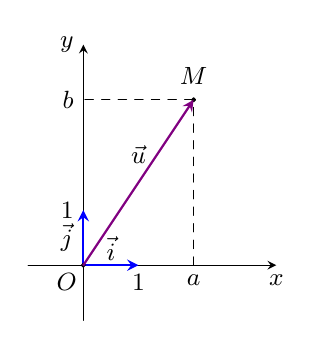
\begin{tikzpicture}[scale=1,font=\small,line join = round, line cap = round, >= stealth, scale = .7]
				      \def\a{-1} \def\b{3.5} \def\c{-1} \def\d{4}
				      \coordinate (O) at (0,0);
				      \coordinate (M) at (2,3);
				      \draw[dashed] (2,0)|-(0,3);
				      \draw[->] (\a,0)--(\b,0)node[below]{$x$};
				      \draw[->] (0,\c)--(0,\d)node[left]{$y$};
				      \draw[->,blue,thick](0,0)--(1,0);
				      \draw[->,blue,thick](0,0)--(0,1);
				      \draw(0.5,0.3) node[]{$\vec{i}$};
				      \draw(-0.3,0.5) node[]{$\vec{j}$};
				      \draw (2,0)node[below]{$a$} (0,3)node[left]{$b$}
				      ;
				      \draw (1,0)node[below]{$1$};
				      \draw (0,1) node[left]{$1$};
				      \foreach \p/\g in {O/-135,M/90} \draw[fill] (\p) circle(1pt)node [shift={(\g:.3)}] {$\p$};
				      \draw[violet,thick,->](O)--(M);
				      \draw (1,2)node[]{$\vec{u}$};
			      \end{tikzpicture}
		      \end{center}
		\item Toạ độ vectơ $\vec{OM}$ là toạ độ điểm $M$
		      \begin{center}
			      \fbox{$M(a;b) \Leftrightarrow \vec{OM}=(a;b)$}
		      \end{center}
		\item Với mỗi vectơ $\vec{u}$, toạ độ vectơ $\vec{u}$ là toạ độ điểm $M$ trong đó $\vec{OM}=\vec{u}$.
	\end{itemize}
\end{dn}
\textbf{Chú ý}.
\begin{itemize}
	\item Vectơ $\vec{i}$ có điểm gốc là $O$ và có toạ độ $(1;0)$ được gọi là \textit{vectơ đơn vị} trên trục $Ox$.
	\item Vectơ $\vec{j}$ có điểm gốc là $O$ và có toạ độ $(0;1)$ được gọi là \textit{vectơ đơn vị} trên trục $Oy$.
\end{itemize}
\begin{dl}
	Trong mặt phẳng toạ độ, ta có:
	\begin{center}
		\fbox{$\vec{u}=a\vec{i}+b\vec{j} \Leftrightarrow \vec{u}=(a;b)$}
	\end{center}
\end{dl}
\textbf{Nhận xét}. Hai vectơ bằng nhau khi và chỉ khi chúng có cùng tọa độ.
\[\vec{u}(x;y)=\vec{v}(x';y')\Leftrightarrow\heva{&x=x'\\&y=y'.} \]
\begin{dn}
	Trong mặt phẳng toạ độ $Oxy$ cho hai điểm $A(x_A;y_A)$ và $B(x_B;y_B)$. Khi đó \fbox{$\overrightarrow{AB}=(x_B-x_A;y_B-y_A)$}.
\end{dn}
\subsubsection{Biểu thức tọa độ của các phép toán vectơ}
\begin{dl}
	Cho hai vectơ $\vec{u}=(x;y)$ và $\vec{v}=(x';y')$. Khi đó
	\begin{itemize}
		\item $\vec{u}+\vec{v}=(x+x';y+y')$
		\item $\vec{u}-\vec{v}=(x-x';y-y')$
		\item $k\vec{u}=(kx;ky)$, với $k\in\mathbb{R}$
	\end{itemize}
\end{dl}
\textbf{Nhận xét.}
\begin{itemize}
	\item Vectơ $\vec{v}(x';y')$ cùng phương với vectơ $\vec{u}(x;y)\neq \vec{0}$ khi và chỉ khi tồn tại số $k$ sao cho $x'=kx$, $y'=ky$ (hay là $\dfrac{x'}{x}=\dfrac{y'}{y}$ nếu $xy\neq 0$).
	\item Trung điểm $M$ của đoạn thẳng $AB$ có tọa độ là $\left(\dfrac{x_A+x_B}{2};\dfrac{y_A+y_B}{2}\right)$.
	\item Trọng tâm $G$ của tam giác $ABC$ có tọa độ là $\left(\dfrac{x_A+x_B+x_C}{3};\dfrac{y_A+y_B+y_C}{3}\right)$.
\end{itemize}
\subsubsection{Biểu thức tọa độ của tích vô hướng}
\begin{dn}{}
	Cho $\overrightarrow{a} = (a_1; a_2)$, $\overrightarrow{b} = (b_1; b_2)$. Khi đó tích vô hướng của hai vectơ $\overrightarrow{a}$ và $\overrightarrow{b}$ được tính theo công thức sau $\overrightarrow{a} \cdot \overrightarrow{b} = a_1b_1 + a_2b_2$.
\end{dn}
\textbf{Nhận xét}
\begin{itemize}
	\item Hai vectơ $\overrightarrow{a}$ và $\overrightarrow{b}$ vuông góc với nhau khi và chỉ khi $a_1b_1 + a_2b_2 = 0$.
	\item Bình phương vô hướng của $\overrightarrow{a}(a_1;a_2)$ là $\overrightarrow{a}^2 = a_1^2 + a_2^2$. \\
	      Suy ra độ dài của $\vec{a}$ bằng $|\vec{a}|=\sqrt{a_1^2+a_2^2}$.
	\item Với hai điểm $A(x_A;y_A)$ và $B(x_B;y_B)$ thì $\overrightarrow{AB}=(x_B-x_A;y_B-y_A)$ và khoảng cách giữa hai điểm $A$, $B$ là $AB=\left|\overrightarrow{AB}\right|=\sqrt{(x_B-x_A)^2+(y_B-y_A)^2}$.
	\item Nếu $\overrightarrow{a}\neq \overrightarrow{0}$ và $\overrightarrow{b}\neq \overrightarrow{0}$ thì $\cos \left(\overrightarrow{a},\overrightarrow{b}\right)= \dfrac{\overrightarrow{a}\cdot \overrightarrow{b} }{ |\overrightarrow{a}|\cdot |\overrightarrow{b}| } = \dfrac{a_1b_1 + a_2b_2}{\sqrt{a_1^2+a_2^2}\cdot \sqrt{b_1^2+b_2^2}}$.
\end{itemize}
\subsection{Các ví dụ}
\begin{vd}%[BG Toán 10(2022)]%[Trần Hòa]%[0H1Y4-3]
	Viết tọa độ các vectơ sau
	$\vec{a}=3\vec{i}+7\vec{j}$; \quad $\vec{b}=\sqrt{2}\vec{i}-3\vec{j}$;\quad $\vec{c}=\dfrac{3}{4}\vec{i}$;\quad$\vec{d}=\pi\vec{j}$.
	\loigiai{
		Ta có $\vec{a}=(3;7)$, $\vec{b}=\left(\sqrt{2};-3\right)$, $\vec{c}=\left(\dfrac{3}{4};0\right)$, $\vec{d}=(0;\pi)$.
	}
\end{vd}
\begin{vd}%[BG Toán 10(2022)]%[Trần Hòa]%[0H1Y4-3]
	Viết vectơ $\vec{u}$ dưới dạng $\vec{u}=x\vec{i}+y\vec{j}$ khi biết tọa độ của $\vec{u}$ là\\
	$(5;3)$, $(2;-1)$, $(4;0)$, $\left(0;-\sqrt{3}\right)$, $(0;0)$.
	\loigiai{
		Ta có $\vec{u}=5\vec{i}+3\vec{j}$, $\vec{u}=2\vec{i}-\vec{j}$, $\vec{u}=4\vec{i}$, $\vec{u}=-\sqrt{3}\vec{j}$, $\vec{u}=0\vec{i}+0\vec{j}=\vec{0}$.
	}
\end{vd}
\begin{vd}%[BG Toán 10(2022)]%[Trần Hòa]%[0H1Y4-2]
	Trong mặt phẳng tọa độ $Oxy$, cho $\vec{u}=(1;2)$, $\vec{v}=(-3;4)$, $\vec{a}=(4;8)$
	\begin{enumerate}
		\item Hãy biểu  thị mỗi vectơ $\vec{u}$, $\vec{v}$, $\vec{a}$ theo các vectơ $\vec{i}$, $\vec{j}$.
		\item Tìm tọa độ $\vec{u}+\vec{v}$, $2\vec{u}$.
		\item Tìm mối liên hệ giữa vectơ $\vec{a}$ và $\vec{u}$.
	\end{enumerate}
	\loigiai{
		\begin{enumerate}
			\item Ta có $\vec{u}=\vec{i}+2\vec{j}$, $\vec{v}=-3\vec{i}+4\vec{j}$, $\vec{a}=6\vec{i}+8\vec{j}$.
			\item Ta có $\vec{u}+\vec{v}=(-2;6)$, $2\vec{u}=(2;4)$.
			\item Ta có $\vec{a}=4\vec{u}$.
		\end{enumerate}
	}
\end{vd}
\begin{vd}%[BG Toán 10(2022)]%[Trần Hòa]%[0H1Y4-2]
	Cho $\vec{u}=(2;-1)$, $\vec{v}=(4;5)$. Tính tọa độ các vectơ $\vec{u}+\vec{v}$, $\vec{u}-\vec{v}$, $3\vec{u}$, $5\vec{u}-4\vec{v}$.
	\loigiai{
		Ta có $\vec{u}+\vec{v}=(6;4)$, $\vec{u}-\vec{v}=(-2;-6)$, $3\vec{u}=(6;-3)$.\\
		Ta có $5\vec{u}=(10;-5)$, $4\vec{v}=(16;20)$ nên $5\vec{u}-4\vec{v}=(-6;-25)$.
	}
\end{vd}

\begin{vd}%[BG Toán 10(2022)]%[Trần Hòa]%[0H1B4-3]
	Cho tam giác $ABC$ có $A(-5;6)$, $B(-4;-1)$, $C(4;3)$.
	\begin{enumerate}
		\item Tìm tọa độ trung điểm $I$ của đoạn thẳng $AC$.
		\item Tìm tọa độ điểm $D$ sao cho tứ giác $ABCD$ là hình bình hành.
	\end{enumerate}
	\loigiai{
		\begin{enumerate}
			\item Gọi $I(x_I;y_I)$. Vì $I$ là trung điểm của của $AC$ nên
			      \[\heva{&x_I=\dfrac{x_A+x_C}{2}=\dfrac{-5+4}{2}=-\dfrac{1}{2}\\&y_I=\dfrac{y_A+y_C}{2}=\dfrac{6+3}{2}=\dfrac{9}{2}.}\] Vậy $I\left(-\dfrac{1}{2};\dfrac{9}{2}\right)$.
			\item Gọi $D(x;y)$, ta có $\overrightarrow{AB}=(1;-7)$, $\overrightarrow{DC}=(4-x;3-y)$.
			      \immini{$ABCD$ là hình bình hành khi $\overrightarrow{AB}=\overrightarrow{CD}\\\Leftrightarrow\heva{&1=4-x\\&-7=3-y}\Leftrightarrow\heva{&x=3\\&y=10} $. Vậy $D(3;10)$.}{\begin{tikzpicture}[scale=1,font=\footnotesize,line join = round, line cap = round, >= stealth]
					      \coordinate (A) at (0,0);
					      \def\a{3} \def\b{2}
					      \coordinate (B) at ($(A)+(0:\a)$);
					      \coordinate (D) at ($(A)+(70:\b)$);
					      \coordinate (C) at ($(B)+(D)-(A)$);
					      \draw (A)--(B)--(C)--(D)--cycle;
					      \foreach \p/\g in {A/-90,B/-90,C/90,D/90} \draw[fill] (\p) circle(.5pt) node [shift={(\g:.3)}] {$\p$};
				      \end{tikzpicture}}
		\end{enumerate}
	}
\end{vd}
\begin{vd}%[BG Toán 10(2022)]%[Trần Hòa]%[0H1B4-3]
	Cho tam giác $ABC$ biết $A(1;-1)$, $B(0;3)$ và $G\left(\dfrac{1}{3};3\right)$ là trọng tâm. Tìm tọa độ điểm $C$.
	\loigiai{
	Gọi $C(x;y)$. Vì $G$ là trọng tâm tam giác $ABC$ nên
	{\allowdisplaybreaks
	\begin{eqnarray*}
		& &\heva{&x_G=\dfrac{x_A+x_B+x_C}{3}\\&y_G=\dfrac{y_A+y_B+y_C}{3}}\\
		&\Rightarrow&
		\heva{&\dfrac{1}{3}=\dfrac{1+0+x}{3}\\&3=\dfrac{-1+3+y}{3}}\\
		&\Rightarrow& \heva{&x=0\\&y=7.}
	\end{eqnarray*}Vậy $C(0;7)$.
	}
	}
\end{vd}
\begin{vd}%[BG Toán 10(2022)]%[Trần Hòa]%[0H1B4-4]
	Cho $\vec{a}=(1;2)$, $\vec{b}=(3;-1)$. Hãy phân tích vectơ $\vec{c}=(-1;5)$ theo hai vectơ $\vec{a}$ và $\vec{b}$.
	\loigiai{
		Giả sử $\vec{c}=k\vec{a}+m\vec{b}=(k+3m;2k-m)$.\\
		Ta có $\heva{&k+3m=-1\\&2k-m=5}\Rightarrow \heva{&k=2\\&m=-1.}$\\ Vậy $\vec{c}=2\vec{a}-\vec{b}$.
	}
\end{vd}
\begin{vd}%[BG Toán 10(2022)]%[Trần Hòa]%[0H1B4-5]
	Cho ba điểm $A(1;-1)$, $B(3;5)$, $C(2;2)$.
	\begin{enumerate}
		\item Chứng minh rằng ba điểm $A$, $B$, $C$ thẳng hàng.
		\item Tìm tọa độ điểm $D$ trên $Ox$ sao cho $A$, $B$, $D$ thẳng hàng.
	\end{enumerate}
	\loigiai{
		\begin{enumerate}
			\item Ta có $\overrightarrow{AB}=(2;6)$, $\overrightarrow{AC}=(1;3)$.\\
			      Vì $\dfrac{2}{1}=\dfrac{6}{3}$ nên $\overrightarrow{AB}$ và $\overrightarrow{AC}$ cùng phương do đó ba điểm $A$, $B$, $C$ thẳng hàng.
			\item Vì $D\in Ox$ nên $D(x;0)$. Ta có $\overrightarrow{AB}=(2;6)$, $\overrightarrow{AD}=(x-1;1)$.\\
			      Ba điểm $A$, $B$, $D$ thẳng hàng khi $\dfrac{x-1}{2}=\dfrac{1}{6}\Rightarrow x-1=\dfrac{1}{3}\Rightarrow x=\dfrac{4}{3}$. Vậy $D\left(\dfrac{4}{3};0\right)$.
		\end{enumerate}
	}
	\loigiai{

	}
\end{vd}
\begin{vd}%[BG Toán 10(2022)]%[Trần Hòa]%[0H2B2-2]
	Cho $A(1;2)$, $B(-2;1)$, $C(2;-1)$.
	\begin{enumerate}
		\item Chứng minh tam giác $ABC$ vuông tại $A$.
		\item Tính diện tích tam giác $ABC$.
	\end{enumerate}
	\loigiai{
		\begin{enumerate}
			\item Ta có $\overrightarrow{AB}=(-3;1)$, $\overrightarrow{AC}=(1;-3)$, $\overrightarrow{BC}=(4;-2)$.\\
			      Suy ra $AB=\sqrt{(-3)^2+1}=\sqrt{10}$, $AC=\sqrt{1^2+(-3)^2}=\sqrt{10}$, $BC=\sqrt{4^2+(-2)^2}=\sqrt{20}$.\\
			      Ta thấy $AB^2+AC^2=10+10=20=BC^2$ nên tam giác $ABC$ vuông tại $A$.
			\item Vì tam giác $ABC$ vuông tại $A$ nên diện tích là $\dfrac{1}{2}AB\cdot AC=\dfrac{1}{2}\cdot \sqrt{10}\cdot \sqrt{10}=5$.
		\end{enumerate}
	}
\end{vd}
\begin{vd}
	Cho các vectơ $\overrightarrow{a}=-\overrightarrow{i}+\overrightarrow{j}, \overrightarrow{b}=\overrightarrow{i}+3\overrightarrow{j}$. Tìm góc giữa hai vectơ $\overrightarrow{a}$ và $\overrightarrow{b}$.
	\loigiai{
		Ta có $\cos (\overrightarrow{a},\overrightarrow{b})=\dfrac{\overrightarrow{a}\cdot \overrightarrow{b}}{\big|\overrightarrow{a}\big|\cdot \big|\overrightarrow{b}\big|}=\dfrac{-1\cdot 1+1\cdot 3}{\sqrt{(-1)^2+1^2}\cdot \sqrt{1^2+3^2}}=\dfrac{2}{2\sqrt{5}}=\dfrac{1}{\sqrt{5}}$.\\
		Do đó góc giữa hai vectơ $\overrightarrow{a}$ và $\overrightarrow{b}$ là góc $\alpha \in [0^\circ;180^\circ]$ sao cho $\cos \alpha =\dfrac{1}{\sqrt{5}}$ hay $ \alpha \approx 65^\circ 26' $.
	}
\end{vd}

\begin{vd}
	Trong mặt phẳng với hệ tọa độ $Oxy$, cho điểm $A(1;3)$ và $B(3;-1)$. Tính góc giữa đường thẳng $OA$ và $AB$.
	\loigiai{
		Ta có $\overrightarrow{AO}=(-1;-3)$ và $\overrightarrow{AB}=(2;-4)$.\\
		Suy ra $\cos\left (\overrightarrow{AO},\overrightarrow{AB}\right )=\dfrac{\overrightarrow{AO}\cdot \overrightarrow{AB}}{AO\cdot AB}=\dfrac{-1\cdot 2+(-3)\cdot (-4)}{\sqrt{10}\cdot \sqrt{20}}=\dfrac{1}{\sqrt{2}}$.\\
		Góc giữa hai vectơ $\overrightarrow{AO}$ và $\overrightarrow{AB}$ bằng góc $\widehat{BAO}=45^\circ$. Do đó góc giữa đường thẳng $OA$ và đường thẳng $AB$ bằng $45^\circ$.
	}
\end{vd}

\begin{vd}%[Lê Nguyễn Viết Tường,BG10-2022]%[0H2B2-3]
	Cho tam giác $ABC$ có $A(2;4)$, $B(2;-2)$, $C(-4;1)$. Tìm tọa độ trực tâm $H$ của tam giác $ABC$.
	\loigiai
	{
		Ta có $\overrightarrow{BC}=(-6;3)$, $\overrightarrow{AB}=(0;-6)$.\\
		Giả sử tọa độ trực tâm $H$ của $\triangle ABC$ là $H(x;y)$, ta có
		\begin{eqnarray*}
			\heva{& AH\perp BC\\&CH\perp AB }\Leftrightarrow\heva{& \overrightarrow{AH}\cdot\overrightarrow{BC}=0\\&\overrightarrow{CH}\cdot\overrightarrow{AB}=0 }\Leftrightarrow\heva{& -6(x-2)+3(y-4)=0\\&0(x+4)-6(y-1)=0 }\Leftrightarrow\heva{& x=\dfrac{1}{2}\\&y=1}.
		\end{eqnarray*}
		Vậy trực tâm của tam giác $ABC$ là $H\left (\dfrac{1}{2};1 \right )$.
	}
\end{vd}
\subsection{Bài tập vận dụng}
\begin{bt}%[0H1B3-1]
	Trong mặt phẳng tọa độ $Oxy$ cho các vectơ $\vec{a}=(3;1)$, $\vec{b}=(-1;2)$. Tính $\vec{u}=3\vec{a}-2\vec{b}$.
	\loigiai{
		Ta có $3\vec{a}=(9;3)$ và $-2\vec{b}=(2;-4)$ nên $\vec{u}=3\vec{a}-2\vec{b}=(11;-1)$.
	}
\end{bt}

\begin{bt}%[0H1B4-4]
	Trong mặt phẳng $Oxy$, cho các vectơ $\overrightarrow{a}=(2;-1),\overrightarrow{b}=(0;4)$ và $\overrightarrow{c}=(3;3)$. Tìm hai số thực $m$, $n$ sao cho $\overrightarrow{c}=m\overrightarrow{a}-n\overrightarrow{b}$.
	\loigiai
	{
		Ta có $m\overrightarrow{a}=(2m;-m),n\overrightarrow{b}=(0;4n) \Rightarrow m\overrightarrow{a}-n\overrightarrow{b}=(2m;-m-4n)$.\\
		Mà $\overrightarrow{c}=m\overrightarrow{a}-n\overrightarrow{b} \Leftrightarrow \heva{&3=2m \\& 3=-m-4n}\Leftrightarrow \heva{&m=\dfrac{3}{2} \\& n=-\dfrac{9}{8}.}$
	}
\end{bt}

\begin{bt}%[0H1B4-3]
	Trong mặt phẳng tọa độ $Oxy$ cho tam giác $ABC$ có $A(-2;3)$, $B(1;2)$, $C(-1;-4)$.
	\begin{enumerate}
		\item Tìm tọa độ điểm $G$ là trọng tâm tam giác $ABC$. Tính chu vi tam giác $ABC$.
		\item Tìm tọa độ điểm $K$ thuộc đoạn thẳng $BC$ sao cho $2KB=3KC$.
	\end{enumerate}
	\loigiai
	{
		\begin{enumerate}
			\item Điểm $G$ là trọng tâm tam giác $ABC$ nên $\heva{&x_G=\dfrac{x_A+x_B+x_C}{3}=-\dfrac{2}{3}\\&y_G=\dfrac{y_A+y_B+y_C}{3}=\dfrac{1}{3}}\Rightarrow G\left(-\dfrac{2}{3};\dfrac{1}{3}\right)$.\\
			      Ta có $\heva{&\overrightarrow{AB}=(3;-1)\Rightarrow AB=\sqrt{3^2+(-1)^2}=\sqrt{10} \\&\overrightarrow{BC}=(-2;-6)\Rightarrow BC=\sqrt{(-2)^2+(-6)^2}=2\sqrt{10}\\&\overrightarrow{CA}=(-1;7)\Rightarrow CA=\sqrt{(-1)^2+7^2}=5\sqrt{2}}\Rightarrow P_{ABC}=3\sqrt{10}+5\sqrt{2}$.
			\item $K$ thuộc đoạn $BC$ nên
			      \begin{eqnarray*}
				      2\overrightarrow{KB}+3\overrightarrow{KC}=\overrightarrow{0}&\Leftrightarrow &  2\left(\overrightarrow{OB}-\overrightarrow{OK}\right)+3\left(\overrightarrow{OC}-\overrightarrow{OK}\right)=\overrightarrow{0}\\
				      &\Rightarrow & \overrightarrow{OK}=\dfrac{2\overrightarrow{OB}+3\overrightarrow{OC}}{5}\\
				      &\Rightarrow & \heva{&x_K=\dfrac{2x_B+3x_C}{5}=-\dfrac{1}{5}\\&y_K=\dfrac{2y_B+3y_C}{5}=-\dfrac{8}{5}.}
			      \end{eqnarray*}

			      Vậy tọa độ cần tìm là $K\left(-\dfrac{1}{5};-\dfrac{8}{5}\right).$
		\end{enumerate}

	}
\end{bt}
\begin{bt}%[0H1B4-5]%[0H2K2-3]%[0H2K2-2]
	Trong mặt phẳng hệ tọa độ $Oxy$, cho ba điểm $A(-1;3)$, $B(-4;-5)$ và $C(1;-2)$.
	\begin{enumerate}
		\item Chứng tỏ $A$, $B$, $C$ là ba đỉnh của một tam giác và tìm tọa độ trọng tâm $G$ của tam giác $ABC$.
		\item Tìm tọa độ trực tâm $H$ của tam giác $ABC$.
		\item Tìm tọa độ điểm $M$ thuộc trục hoành sao cho $\left|2\overrightarrow{MA}+\overrightarrow{MC}\right|$ đạt giá trị nhỏ nhất.
	\end{enumerate}
	\loigiai{
		\begin{enumerate}
			\item Ta có $\overrightarrow{AB}=(-3;-8)$, $\overrightarrow{AC}=(2;-5)$.\\
			      Vì $\dfrac{-3}{2}\ne \dfrac{-8}{-5}$ nên hai vectơ $\overrightarrow{AB}$ và $\overrightarrow{AC}$ không cùng phượng. Từ đó suy ra  $A$, $B$, $C$ là ba đỉnh của một tam giác.\\
			      Tọa độ trọng tâm $G$ của tam giác $ABC$ là
			      \begin{eqnarray*}
				      \heva{&x_G=\dfrac{x_A+x_B+x_C}{3}=\dfrac{(-1)+(-4)+1}{3}=-\dfrac{4}{3}\\&y_G=\dfrac{y_A+y_B+y_C}{3}=\dfrac{3+(-5)+(-2)}{3}=-\dfrac{4}{3}}
			      \end{eqnarray*}
			      Vậy $G\left(-\dfrac{4}{3};-\dfrac{4}{3}\right)$.
			\item Giả sử $H(x;y)$ là trực tâm của tam giác $ABC$.\\
			      Ta có $\overrightarrow{BH}=(x+4;y+5)$, $\overrightarrow{CH}=(x-1;y+2)$, $\overrightarrow{AB}=(-3;-8)$, $\overrightarrow{AC}=(2;-5)$.\\
			      Vì $H$ là trực tâm tam giác $ABC$ nên
			      \begin{eqnarray*}
				      \heva{&\overrightarrow{AB}\perp\overrightarrow{CH}\\&\overrightarrow{AC}\perp\overrightarrow{BH}}
				      &\Leftrightarrow & \heva{&\overrightarrow{AB}\cdot\overrightarrow{CH}=0\\&\overrightarrow{AC}\cdot\overrightarrow{BH}=0}\\
				      &\Leftrightarrow & \heva{&(-3)\cdot(x-1)+(-8)\cdot (y+2)=0\\&2\cdot (x+4)+(-5)\cdot (y+5)=0}\\
				      &\Leftrightarrow & \heva{&3x+8y=-13\\&2x-5y=17}\\
				      &\Leftrightarrow & \heva{&x=\dfrac{71}{31}\\&y=-\dfrac{77}{31}.}
			      \end{eqnarray*}
			      Vậy $H\left(\dfrac{71}{31};-\dfrac{77}{31}\right)$.
			\item Gọi $M(x;0)$ là điểm thuộc trục hoành, ta có
			      \begin{eqnarray*}
				      \heva{&\overrightarrow{MA}=(-1-x;3)\\&\overrightarrow{MC}=(1-x;-2)}\Rightarrow 2\overrightarrow{MA}+\overrightarrow{MC}=(-1-3x;4).
			      \end{eqnarray*}
			      Nên
			      \begin{eqnarray*}
				      \left|2\overrightarrow{MA}+\overrightarrow{MC}\right|& =&\sqrt{(-1-3x)^2+4^2}\\
				      & =&\sqrt{(1+3x)^2+4^2}\ge 4.
			      \end{eqnarray*}
			      Dấu ``$=$'' xảy ra khi và chỉ khi $1+3x=0 \Leftrightarrow x=-\dfrac{1}{3}$. Khi đó $M\left(-\dfrac{1}{3};0\right)$.
		\end{enumerate}
	}
\end{bt}

\begin{bt}%[0H1B4-3]
	Trong mặt phẳng $Oxy$ cho ba điểm $A(3; 4)$, $B(2; 1)$, $C(6; 3)$. Tìm tọa độ điểm $N$ thỏa mãn $2 \overrightarrow{NB}+ \overrightarrow{NC}- \overrightarrow{NA}= \overrightarrow{0}$.
	\loigiai{
		Giả sử $N(x;y)$.
		Ta có $\overrightarrow{NB}= (2-x; 1-y), \overrightarrow{NC}= (6-x; 3-y), \overrightarrow{NA}= (3-x; 4-y)$.\\
		Khi đó
		\begin{align*}
			2 \overrightarrow{NB}+ \overrightarrow{NC}- \overrightarrow{NA}= \overrightarrow{0} & \Leftrightarrow \heva{ & 2(2-x)+(6-x)- (3-x)=0 \\ &2(1-y)+ (3-y)- (4-y)=0}\\
			                                                                                    & \Leftrightarrow \heva{ & 7-2x=0                \\ &1-2y=0} \Leftrightarrow \heva{&x= \dfrac{7}{2}\\ &y= \dfrac{1}{2}.}
		\end{align*}
		Vậy, $N \left(\dfrac{7}{2}; \dfrac{1}{2}\right)$ là điểm cần tìm.
	}
\end{bt}
\begin{bt}%[0H1B4-3]
	Trong mặt phẳng tọa độ $Oxy$, cho ba điểm $M(-1;1)$, $N\left(1;3\right)$, $P(-2;5).$
	Tìm tọa độ điểm $E$ biết $\overrightarrow{PE}=2\overrightarrow{MN}$.
	\loigiai{Ta có $\overrightarrow{MN}=(2;2)$.\\
		$\overrightarrow{PE}=2\overrightarrow{MN}\Leftrightarrow \heva{
				& x_E+2=4 \\
				& y_E-5=4 \\
			}\Leftrightarrow \heva{
				& x_E=2 \\
				& y_E=9. \\}$\\
		Vậy $E(2;9)$.
	}
\end{bt}
\begin{bt}%[0H1B4]%
	Trong mặt phẳng với hệ tọa độ $Oxy$, cho tam giác $ABC$ với $A\left(1;1\right)$, $B\left(2;3\right)$, $C\left(5;-1\right)$. Tìm tọa độ điểm $D$ sao cho tứ giác $ABDC$ là hình bình hành.
	\loigiai{
		Tứ giác $ABDC$ là hình bình hành $\Leftrightarrow \overrightarrow{AB} = \overrightarrow{CD} \Leftrightarrow \heva{&x_D - 5 = 1 \\&y_D + 1 = 2} \Leftrightarrow \heva{&x_D = 6 \\ &y_D = 1}.$ \\
		Vậy $D(6;1)$ là điểm cần tìm.
	}
\end{bt}
\begin{bt}%[0H1B4-3]%[0H1K4-3]
	Trong mặt phẳng $Oxy$, cho $M(3;-1)$, $N(1;2)$ và $P(2;-4)$.
	\begin{enumerate}
		\item Tìm tọa độ trọng tâm $G$ của tam giác $MNP$ và tọa độ điểm $Q$ sao cho tứ giác $MNGQ$ là hình bình hành.
		\item Tam giác $ABC$ nhận các điểm $M$, $N$, $P$ lần lượt là trung điểm của các cạnh $AB$, $BC$, $CA$. Tìm tọa độ các điểm $A$, $B$, $C$.
	\end{enumerate}
	\loigiai
	{
		\immini
		{\begin{enumerate}
				\item Tọa độ trọng tâm $G$ của tam giác $MNP$ là
				      \[G=\left(\dfrac{3+1+2}{3};\dfrac{-1+2-4}{3}\right)=\left(2;-1\right).\]
				      Gọi $Q(x;y)$.\\
				      Vì tứ giác $MNGQ$ là hình bình hành nên $\overrightarrow{MQ}=\overrightarrow{NG}.\hfill(1)$\\
				      Ta có $\overrightarrow{MQ}=(x-3;y+1)$ và $\overrightarrow{NG}=(1;-3)$.
				      Từ (1) suy ra
				      \[\heva{&x-3=1\\&y+1=-3}\Leftrightarrow\heva{&x=4\\&y=-4.}\]
				      Vậy $Q(4;-4)$.
				\item Gọi $C(c_1;c_2)$, theo đề bài thì tứ giác $MNCP$ là hình bình hành nên
				      \[\heva{&c_1+x_M=x_N+x_P\\&c_2+y_M=y_N+y_P}\Leftrightarrow\heva{&c_1=1+2-3=0\\&c_2=2+(-4)-(-1)=-1.}\]
				      Vậy $C(0;-1)$.\\
				      Gọi $B(b_1;b_2)$, vì $N$ là trung điểm $CB$ nên
				      \[\heva{&b_1=2x_N-c_1\\&b_2=2y_N-c_2}\Leftrightarrow\heva{&b_1=2\cdot1-0=2\\&b_2=2\cdot2-(-1)=5.}\]
				      Vậy $B(2;5)$.\\
				      Gọi $A(a_1;a_2)$, vì $M$ là trung điểm $AB$ nên
				      \[\heva{&a_1=2x_M-b_1\\&a_2=2y_M-b_2}\Leftrightarrow\heva{&a_1=2\cdot3-2=4\\&a_2=2\cdot(-1)-5=-7.}\]
				      Vậy $A(4;-7)$.
			\end{enumerate}}
		{\begin{tikzpicture}[line cap=round,line join=round,font=\footnotesize,>=stealth,scale=0.75]
				\fill (3,-1) coordinate [label=right:$M$] (M) circle(1pt)
				(1,2) coordinate [label=left:$N$] (N) circle(1pt)
				(2,-4) coordinate [label=below left:$P$] (P) circle(1pt);
				\tkzCentroid(M,N,P)\tkzGetPoint{G};
				\coordinate (Q) at ($(M)+(G)-(N)$);
				\coordinate (B) at ($(N)+(M)-(P)$);
				\coordinate (C) at ($(N)+(P)-(M)$);
				\coordinate (A) at ($2*(P)-(C)$);
				\fill (G) node[right]{$G$} circle(1pt)
				(Q) node[below]{$Q$} circle(1pt)
				(B) node[above]{$B$} circle(1pt)
				(C) node[left]{$C$} circle(1pt)
				(A) node[below]{$A$} circle(1pt);
				\draw (M)--(N)--(P)--cycle (N)--(G)--(Q)--(M) (B)--(C)--(A)--(B);
			\end{tikzpicture}}
	}
\end{bt}

\begin{bt}%[0H1B4-3]%[0H1K4-3]
	Trong mặt phẳng tọa độ $Oxy$, cho điểm $A(-3;5)$, $B(-4;-3)$, $C(1;1)$.
	\begin{enumerate}
		\item Tìm tọa độ điểm $D$ sao cho tứ giác $ABCD$ là hình bình hành.
		\item Tìm tọa độ điểm $K$ thuộc trục hoành sao cho $KA+KB$ nhỏ nhất.
	\end{enumerate}
	\loigiai{
		%		\begin{center}
		%			\begin{tikzpicture}[>=stealth,line join=round,line cap=round,scale=.5]
		%			\tkzDefPoints{-3/5/A,-4/-3/B,1/1/C}
		%			\tkzDefPointBy[translation=from B to A](C)\tkzGetPoint{D}
		%			\tkzDrawSegments[](A,B B,C C,D D,A)
		%			\tkzLabelPoints[above left	](A)
		%			\tkzLabelPoints[above right](D)
		%			\tkzLabelPoints[below left](B)
		%			\tkzLabelPoints[below right](C)
		%			\end{tikzpicture}
		%		\end{center}
		\begin{enumerate}
			\item Tứ giác $ABCD$ là hình bình hành \\
			      $\Leftrightarrow\overrightarrow{AB}=\overrightarrow{DC}\Leftrightarrow (-1;-8)=(1-x_D;1-y_D)\Leftrightarrow\heva{&1-x_D=-1\\&1-y_D=-8}\Leftrightarrow\heva{&x_D=2\\&y_D=9.}$\\
			      Vậy $D(2;9)$ là điểm cần tìm.
			\item Gọi $K(a;0)$ là điểm cần tìm.\\
			      Ta có $KA+KB\ge AB$.\\
			      Dấu \lq\lq $=$\rq\rq\, xảy ra khi $A,K,B$ thẳng hàng.\\
			      $\Leftrightarrow \overrightarrow{AK}=k\overrightarrow{AB}\Leftrightarrow (a+3;-5)=k(-1;-8)\Leftrightarrow\heva{&a+3=-k\\&-5=-8k}\Leftrightarrow\heva{&a=-\dfrac{29}{8}\\&k=\dfrac{5}{8}.}$\\
			      Vậy $K\left(-\dfrac{29}{8};0\right) $ thỏa yêu cầu bài toán.
		\end{enumerate}
	}
\end{bt}

\begin{bt}
	Trong mặt phẳng tọa độ $ Oxy $, tính góc giữa hai vectơ $ \overrightarrow{a} $ và $ \overrightarrow{b} $ trong mỗi trường hợp sau:
	\begin{multicols}{2}
		\begin{enumerate}
			\item $ \overrightarrow{a}=(4;3) $, $ \overrightarrow{b}=(1;7) $;%\dapso{$ 45^\circ $}
			\item $ \overrightarrow{a}=(2;5) $, $ \overrightarrow{b}=(3;-7) $;%\dapso{$ 135^\circ $}
			\item $ \overrightarrow{a}=(6;-8) $, $ \overrightarrow{b}=(12;9) $;%\dapso{$ 90^\circ $}
			\item $ \overrightarrow{a}=(2;-6) $, $ \overrightarrow{b}=(-3;9) $.%\dapso{$ 180^\circ $}
		\end{enumerate}
	\end{multicols}
	\loigiai{
		\begin{enumerate}
			\item $\cos (\overrightarrow{a},\overrightarrow{b})=\dfrac{\overrightarrow{a}\cdot \overrightarrow{b}}{\big|\overrightarrow{a}\big|\cdot \big|\overrightarrow{b}\big|}=\dfrac{4\cdot 1+3\cdot 7}{\sqrt{4^2+3^2}\cdot \sqrt{1^2+7^2}}=\dfrac{25}{5\sqrt{50}}=\dfrac{1}{\sqrt{2}}$.\\
			      Suy ra góc giữa hai vectơ $ \overrightarrow{a} $ và $ \overrightarrow{b} $ là $ 45^\circ $.
			\item $\cos (\overrightarrow{a},\overrightarrow{b})=\dfrac{\overrightarrow{a}\cdot \overrightarrow{b}}{\big|\overrightarrow{a}\big|\cdot \big|\overrightarrow{b}\big|}=\dfrac{2\cdot 3+5\cdot (-7)}{\sqrt{2^2+5^2}\cdot \sqrt{3^2+(-7)^2}}=\dfrac{-29}{\sqrt{29}\cdot \sqrt{58}}=-\dfrac{1}{\sqrt{2}}$.\\
			      Suy ra góc giữa hai vectơ $ \overrightarrow{a} $ và $ \overrightarrow{b} $ là $ 135^\circ $.
			\item $ \overrightarrow{a}\cdot \overrightarrow{b}=6\cdot 12+(-8)\cdot 9=0 $
			      Suy ra góc giữa hai vectơ $ \overrightarrow{a} $ và $ \overrightarrow{b} $ là $ 90^\circ $.
			\item $\cos (\overrightarrow{a},\overrightarrow{b})=\dfrac{\overrightarrow{a}\cdot \overrightarrow{b}}{\big|\overrightarrow{a}\big|\cdot \big|\overrightarrow{b}\big|}=\dfrac{2\cdot (-3)+(-6)\cdot 9}{\sqrt{2^2+(-6)^2}\cdot \sqrt{(-3)^2+9^2}}=\dfrac{-60}{\sqrt{40}\cdot \sqrt{90}}=-1$.\\
			      Suy ra góc giữa hai vectơ $ \overrightarrow{a} $ và $ \overrightarrow{b} $ là $ 180^\circ $.
		\end{enumerate}
	}
\end{bt}

% \begin{bt}%0H1T4-3
% 	Trong hình sau, quân mã đang ở vị trị có toạ độ $(1;2)$. Hỏi sau một nước đi, quân mã có thể đến những vị trí nào?
% 	\begin{center}
% 		\begin{tikzpicture}[font=\footnotesize, line join=round, line cap=round, >=stealth]
% 			\begin{scope}[scale=0.75]
% 				%Tô màu ô vuông
% 				\foreach \i in{0,1,...,7}
% 				\foreach \j in{0,1,...,7}
% 				{
% 					\pgfmathparse{mod(\i+\j,2)? "yellow!50": "white"}
% 					\fill[\pgfmathresult,draw=black](\i,\j)rectangle(\i+1,\j+1);
% 				}
% 				\foreach \x/\y/\m in{1/3/\BlackKnightOnWhite,5/4/\BlackRookOnWhite,5/8/\BlackRookOnWhite,7/3/\BlackBishopOnWhite,7/5/\BlackBishopOnWhite
% 				}
% 				\path(\x,\y)++(0.5,-0.5)node{\m};
% 				\foreach \x/\y/\m in{1/6/\BlackKingOnWhite,2/5/\BlackRookOnWhite,3/4/\BlackPawnOnWhite}
% 				\path(\x,\y)++(0.5,-0.5)node{\color{red}\m};
% 				\draw[->,line width=1 pt,shift={(0.5,0.5)}](0,0)--(8,0)node[below]{$x$};
% 				\draw[->,line width=1 pt,shift={(0.5,0.5)}](0,0)--(0,8)node[left]{$y$};
% 				\foreach \x in {1,2,...,7}{
% 					\draw[fill=black] (\x,0)++(0.5,0.5)circle(1.5pt)node[below]{$\x$};
% 					\draw[fill=black] (0.5,\x+0.5)circle(1.5pt)++(0,0)node[left]{$\x$};}
% 				\draw[dashed,line width=1 pt](-0.5,0.5)--(0.5,0.5)--(0.5,-0.5);
% 			\end{scope}
% 			\draw (0,0)node[]{O};
% 		\end{tikzpicture}
% 	\end{center}
% 	\loigiai{
% 		Sau một nước đi, quân mã có thể đến một trong những vị trí sau
% 		$\left\lbrace (0;0),(2;0),(3;1),(3;3),(2;4),(0;4)\right\rbrace $.
% 	}
% \end{bt}

\begin{bt}%[Lê Nguyễn Viết Tường,BG10-2022]%[0H2B2-3]
	Trong mặt phẳng tọa độ $Oxy$, cho hai vectơ $\overrightarrow{u}=\left (\dfrac{1}{2};-5 \right )$ và $\overrightarrow{v}=\left (k;-4 \right )$. Tìm $k$ để $\overrightarrow{u}$ vuông góc với $\overrightarrow{v}$.
	\loigiai
	{
		Ta có $\overrightarrow{u}\perp\overrightarrow{v}\Leftrightarrow\overrightarrow{u}\cdot\overrightarrow{v}=0\Leftrightarrow \dfrac{1}{2}k+(-5)(-4)=0\Leftrightarrow k=-40.$
	}
\end{bt}

\begin{bt}%[Lê Nguyễn Viết Tường,BG10-2022]%[0H2B2-3]
	Trong mặt phẳng tọa độ $Oxy$, cho ba vectơ $\overrightarrow{u}=(4;1)$, $\overrightarrow{v}=(1;4)$ và $\overrightarrow{a}=\overrightarrow{u}+m\cdot\overrightarrow{v}$ với $m\in\mathbb{R}$. Tìm $m$ để $\overrightarrow{a}$ vuông góc với trục hoành.
	\loigiai
	{
		Ta có $\overrightarrow{a}=\overrightarrow{u}+m\overrightarrow{v}=\left (4+m;1+4m \right )$.\\
		Trục hoành có vectơ đơn vị là $\overrightarrow{i}=(1;0)$.\\
		$\overrightarrow{a}$ vuông góc với trục hoành $\Leftrightarrow \overrightarrow{a}\cdot\overrightarrow{i}=0\Leftrightarrow 4+m=0\Leftrightarrow m=-4$.
	}
\end{bt}

\begin{bt}%[Lê Nguyễn Viết Tường,BG10-2022]%[0H2B2-3]
	Trong mặt phẳng tọa độ $Oxy$, cho hai điểm $A(-2;4)$ và $B(8;4)$. Tìm tọa độ điểm $C$ thuộc trục hoành sao cho tam giác $ABC$ vuông tại $C$.
	\loigiai
	{
		Ta có $C\in Ox\Rightarrow C(c;0)$ và $\heva{& \overrightarrow{CA}=(-2-c;4)\\&\overrightarrow{CB}=(8-c;4) .}$\\
		$\triangle ABC$ vuông tại $C$ nên $\overrightarrow{CA}\cdot\overrightarrow{CB}=0\Rightarrow (-2-c)(8-c)+4\cdot 4=0\Rightarrow\hoac{& c=6\\&c=0. }$\\
		Vậy $C(6;0)$ hoặc $C(0;0)$.
	}
\end{bt}

\subsection{Bài tập trắc nghiệm}
\Opensolutionfile{ansbook}[ans/ansbook-2D1-1-TN]
\Opensolutionfile{ans}[ans/ans-0H1-1-TN]
\begin{ex}%[Bài giảng Toán 10 2022]%[Phạm Tiến Long]%[0H1Y4-1]
	Trong hệ tọa độ $Oxy$, biết $\overrightarrow{u}=2\overrightarrow{i}-\overrightarrow{j}$. Khi đó $\overrightarrow{u}$ có tọa độ là
	\choice
	{\True $(2;-1)$}
	{$(2;1)$}
	{$(1;2)$}
	{$(1;-2)$}
	\loigiai{
		$\overrightarrow{u}$ có tọa độ là $(2;-1)$.
	}
\end{ex}
\begin{ex}%[Bài giảng Toán 10 2022]%[Phạm Tiến Long]%[0H1Y4-3]
	Trong mặt phẳng tọa độ $Oxy$, tọa độ của $\overrightarrow{i}$ là bao nhiêu?
	\choice
	{$\overrightarrow{i} = (0; 1)$}
	{$\overrightarrow{i} = (-1; 0)$}
	{$\overrightarrow{i} = (0; 0)$}
	{\True $\overrightarrow{i} = (1; 0)$}
	\loigiai{
		Ta có vectơ đơn vị $\overrightarrow{i}=(1;0)$.}
\end{ex}
\begin{ex}%[Bài giảng Toán 10 2022]%[Phạm Tiến Long]%[0H1Y4-3]
	Trong mặt phẳng $Oxy$, cho $A(1;3)$, $B(2;-5)$. Tìm tọa độ của vectơ $\overrightarrow{AB}$.
	\choice
	{$\overrightarrow{AB}=(2;-15)$}
	{$\overrightarrow{AB}=(3;-2)$}
	{$\overrightarrow{AB}=(-1;8)$}
	{\True $\overrightarrow{AB}=(1;-8)$}
	\loigiai{
		Tọa độ $\overrightarrow{AB}=(1;-8)$.
	}
\end{ex}
\begin{ex}%[Bài giảng Toán 10 2022]%[Phạm Tiến Long]%[0H1K4-3]
	Trong mặt phẳng tọa độ $Oxy$, cho ba điểm $A(1;3)$, $B(2;-3)$, $C(-2;1)$. Tìm tọa độ điểm $M$ thỏa mãn $ 5\overrightarrow{MA}-2\overrightarrow{MB}=4\overrightarrow{MC}$.
	\choice
	{$M(3;17)$}
	{$M(-3;-17)$}
	{\True $ M(-9;-17)$}
	{$M(9;17) $}
	\loigiai{
		Giả sử $M(a; b)$.\\
		Ta có:
		$ \heva{
				&\overrightarrow{MA}= (1-a; 3-b)\\
				&\overrightarrow{MB}= (2-a; -3-b)\\
				&\overrightarrow{MC}= (-2-a; 1-b)}$
		$ \Rightarrow
			\heva{
				& 5\overrightarrow{MA}= (5-5a; 15-5b)\\
				& 2 \overrightarrow{MB}= (4-2a; -6-2b)\\
				& 4\overrightarrow{MC}= (-8-4a; 4-4b).}$\\
		Vậy $ 5\overrightarrow{MA}-2\overrightarrow{MB}=4\overrightarrow{MC}$ $\Leftrightarrow
			\heva{
				& 5-5a-4+2a=-8-4a\\
				& 15-5b+6+2b=4-4b}$
		$ \Leftrightarrow
			\heva{
				& a= -9\\
				& b= -17.}$\\
		Vậy $M(-9;-17)$.

	}
\end{ex}
\begin{ex}%[Bài giảng Toán 10 2022]%[Phạm Tiến Long]%[0H1K4-3]
	Trong mặt phẳng tọa độ $Oxy$, cho tam giác $ABC$, biết $B(9;7)$, $C(11;-1)$ và $M(1;2)$ là trung điểm của $AB$. Tìm tọa độ trung điểm $N$ của $AC$.
	\choice
	{\True $N(2;-2)$}
	{$N(-2;8)$}
	{$N(-2;2)$}
	{$N(2;-8)$}
	\loigiai{
		Vì $M(1;2)$ là trung điểm của $AB$ nên ta có $ \heva{&x_A=2x_M-x_B=-7\\&y_A=2y_M-y_B=-3}\Rightarrow A(-7; -3)$.\\
		Mặt khác $N$ là trung điểm của $AC$ nên $\heva{&x_N=\dfrac{x_A+x_C}{2}=2\\&y_N=\dfrac{y_A+y_C}{2}=-2}\Rightarrow N(2;-2)$.
	}
\end{ex}
\begin{ex}%[Bài giảng Toán 10 2022]%[Phạm Tiến Long]%[0H1B4-3]
	Trong mặt phẳng tọa độ $O x y$, cho $A (0; 3)$, $B (4; 2)$. Tìm tọa độ điểm $D$ thỏa mãn $\overrightarrow{OD} - 2 \overrightarrow{DA} + 2 \overrightarrow{DB} = \overrightarrow{0}$.
	\choice
	{\True $(-8; 2)$}
	{$\left(2; \dfrac{5}{2} \right)$}
	{$(-3; 3)$}
	{$(8; -2)$}
	\loigiai{
		Ta có $\overrightarrow{BA} = (-4; 1)$. \\
		$\overrightarrow{OD} - 2 \overrightarrow{DA} + 2 \overrightarrow{DB} = \overrightarrow{0} \Leftrightarrow \overrightarrow{OD} = 2 \overrightarrow{DA} - 2 \overrightarrow{DB} = 2 \overrightarrow{BA} = (-8; 2)$.\\ Suy ra tọa độ điểm $D$ là $(-8; 2)$.
	}
\end{ex}
\begin{ex}%[Bài giảng Toán 10 2022]%[Phạm Tiến Long]%[0H1Y4-3]
	Trong mặt phẳng $Oxy$, cho $A(2;3)$, $B(2;-5)$. Gọi $I$ là trung điểm của đoạn thẳng $AB$. Vectơ $\overrightarrow{AI}$ có tọa độ là
	\choice
	{$(1;-3)$}
	{$(0;5)$}
	{$(0;-2)$}
	{\True $(0;-4)$}
	\loigiai{
		Vì $I$ là trung điểm của đoạn thẳng $AB$ nên điểm $I$ có tọa độ là $(2;-1)$.\\
		Suy ra $\overrightarrow{AI}=(0;-4)$.
	}
\end{ex}
\begin{ex}%[Bài giảng Toán 10 2022]%[Phạm Tiến Long]%[0H1B4-1]
	Cho $A(1; 2)$ và $I(3; 4)$ là trung điểm của đoạn thẳng $AB$. Tọa độ của đỉnh $B$ là
	\choice
	{$(6; 5)$}
	{$(3; 2)$}
	{$(2; 3)$}
	{\True $(5; 6)$}
	\loigiai{
		Ta có $\heva{& x_B = 2x_I - x_A\\&y_B = 2y_I - y_A} \Leftrightarrow \heva{& x_B = 5\\&y_B = 6}$. Vậy $B(5; 6)$.
	}
\end{ex}
\begin{ex}%[Bài giảng Toán 10 2022]%[Phạm Tiến Long]%[0H1B4-3]
	Trong hệ trục tọa độ $Oxy$, cho $A(-4;1)$, $B(2;4)$, $G(2;-2)$. Tìm tọa độ điểm $C$ sao cho $G$ là trọng tâm tam giác $ABC$.
	\choice
	{\True $C(8;-11)$}
	{$C(8;11)$}
	{$C(-8;-11)$}
	{$C(12;11)$}
	\loigiai{
		$G$ là trọng tâm tam giác $ABC$ nên $$\heva{&x_A+x_B+x_C=3x_G\\&y_A+y_B+y_C=3y_G}\Leftrightarrow \heva{&x_C=3x_G-\left(x_A+x_B\right)\\&y_C=3y_G-\left(y_A+y_B\right)}\Leftrightarrow \heva{&x_C=6-(-4+2)=8\\&y_C=-6-(1+4)=-11}\Rightarrow C(8;-11).$$
	}
\end{ex}
\begin{ex}%[Bài giảng Toán 10 2022]%[Phạm Tiến Long]%[0H1K4-3]
	Trong mặt phẳng với hệ tọa độ $Oxy$, cho hai điểm $B(-2;3)$ và $C(3;-2)$. Điểm $I(a;b)$ thuộc $BC$ sao cho với mọi điểm $M$ không nằm trên đường thẳng BC thì $\overrightarrow{MI}=\dfrac{2}{5}\overrightarrow{MB}+\dfrac{3}{5}\overrightarrow{MC}$. Tính $S=a^2+b^2$.
	\choice
	{\True $1$}
	{$0$}
	{$4$}
	{$5$}
	\loigiai{
	Giả sử $\overrightarrow{IB}=k\overrightarrow{IC}$. Khi đó $\overrightarrow{IM}+\overrightarrow{MB}=k\overrightarrow{IM}+k\overrightarrow{MC}\Rightarrow \overrightarrow{MI}=\dfrac{1}{1-k}\overrightarrow{MB}+\dfrac{-k}{1-k}\overrightarrow{MC}$.\\
	Do $\overrightarrow{MI}=\dfrac{2}{5}\overrightarrow{MB}+\dfrac{3}{5}\overrightarrow{MC}$ nên ta có $\heva{& \dfrac{1}{1-k}=\dfrac{2}{5} \\ & \dfrac{-k}{1-k}=\dfrac{3}{5}} \Leftrightarrow k=-\dfrac{3}{2}$.\\
	Vậy $\overrightarrow{BI}=\dfrac{3}{5}\overrightarrow{BC} \Rightarrow \heva{& x_I=x_B+\dfrac{3}{5}x_{BC} \\ & y_I=y_B+\dfrac{3}{5}y_{BC}} \Leftrightarrow \heva{& x_I=1 \\ & y_I=0.} $\\
	Vậy $a^2+b^2=1$.
	}
\end{ex}
\begin{ex}%[Bài giảng Toán 10 2022]%[Phạm Tiến Long]%[0H1B4-3]
	Trong mặt phẳng tọa độ $Oxy$, cho hai vectơ $\overrightarrow{a}=(3;-1)$ và $\overrightarrow{b}=(3;4)$. Tính tọa độ vectơ $\overrightarrow{c}=\overrightarrow{a}+\overrightarrow{b}$.
	\choice
	{$\overrightarrow{c}=(3;3)$}
	{$\overrightarrow{c}=(2;7)$}
	{$\overrightarrow{c}=(2;1)$}
	{\True $\overrightarrow{c}=(6;3)$}
	\loigiai{
		Ta có $\overrightarrow{c}=\overrightarrow{a}+\overrightarrow{b}=(6;3)$.
	}
\end{ex}
\begin{ex}%[Bài giảng Toán 10 2022]%[Phạm Tiến Long]%[0H1G4-3]
	Trong mặt phẳng tọa độ $Oxy$, cho tam giác $ABC$ với $A(1;-2)$, $B(0;-1)$, $C(3;0)$. Tìm tọa độ điểm $G$ sao cho với điểm $M$ bất kì ta luôn có $\overrightarrow{MA}+\overrightarrow{MB}+\overrightarrow{MC}=3\overrightarrow{MG}$.
	\choice
	{$G\left(\dfrac{4}{3};-2\right)$}
	{$G\left(\dfrac{5}{3};-1\right)$}
	{$G\left(\dfrac{7}{3};-2\right)$}
	{\True $G\left(\dfrac{4}{3};-1\right)$}
	\loigiai{
		Ta có $\overrightarrow{MA}+\overrightarrow{MB}+\overrightarrow{MC}=3\overrightarrow{MG}$. Do đó $\overrightarrow{GA}+\overrightarrow{GB}+\overrightarrow{GC}=\overrightarrow{0}$,
		suy ra $G$ là trọng tâm của tam giác $ABC$. Vậy $G\left(\dfrac{4}{3};-1\right)$. }
\end{ex}
\begin{ex}%[Bài giảng Toán 10 2022]%[Phạm Tiến Long]%[0H1B4-3]
	Cho ba điểm $A(2;5)$, $B(1;1)$, $C(3;3)$. Tìm tọa độ điểm $E$ sao cho $\overrightarrow{AE} = 3\overrightarrow{AB} - 2\overrightarrow{AC}$.
	\choice
	{$E(-2;-3)$}
	{$E(3;-3)$}
	{$E(-3;3)$}
	{\True $E(-3;-3)$}
	\loigiai{
		Gọi $E(x_E;y_E)$ là điểm cần tìm.\\
		Ta có
		\begin{eqnarray*}
			& &  \overrightarrow{AE} = (x_E - 2; y_E - 5)\\
			& &  \overrightarrow{AB} = (-1;-4)\\
			& &  \overrightarrow{AC} = (1;-2).
		\end{eqnarray*}
		$\Rightarrow	 3\overrightarrow{AB} - 2\overrightarrow{AC}= (-5;-8)$, do đó
		$$ \overrightarrow{AE} = 3\overrightarrow{AB} - 2\overrightarrow{AC} \Leftrightarrow \heva{&x_E - 2 = -5\\&y_E - 5 = - 8} \Leftrightarrow \heva{&x_E = -3\\&y_E = -3} \Rightarrow E(-3;-3).$$
	}
\end{ex}
\begin{ex}%[Bài giảng Toán 10 2022]%[Phạm Tiến Long]%[0H1K4-3]
	Trong mặt phẳng $Oxy$, cho tam giác $MNP$ có $M(1; -1)$,  $N(5; -3)$ và $P$ thuộc trục $Oy$, trọng tâm $G$ của tam giác $MNP$ nằm trên trục $Ox$. Tìm toạ độ của điểm $P$.
	\choice
	{$P(0; 2)$}
	{$P(0; 10)$}
	{\True $P(0; 4)$}
	{$P(2; 0)$}
	\loigiai{
		Do $P \in Oy$ nên $P(0; y_P)$.\\
		Trọng tâm $G \in Ox$ nên $G(x_G; 0)$.\\
		Do $G$ là trọng tâm của tam giác $MNP$ nên $\heva{& x_M + x_N + x_P = 3x_G \\ & y_M + y_N + y_P = 3y_G.}$\\
		Khi đó $\heva{& 1 + 5 + 0 = 3x_G\\& -1 - 3 + y_P = 0} \Leftrightarrow \heva{& x_G = 6\\ & y_P = 4.}$\\
		Vậy $P(0; 4)$.}
\end{ex}
\begin{ex}%[Bài giảng Toán 10 2022]%[Phạm Tiến Long]%[0H1K4-3]
	Trong mặt phẳng tọa độ $Oxy$, tìm tọa độ điểm $M$ trên trục hoành sao cho $A$, $B$, $M$ thẳng hàng với $A(2;-3)$ và $B(3;4)$.
	\choice
	{$(1;0)$}
	{\True $\left(\dfrac{17}{7};0\right)$}
	{$\left(-\dfrac{5}{3};0\right)$}
	{$(4;0)$}
	\loigiai{
		Vì điểm $M$ nằm trên trục hoành nên ta giả sử $M$ có tọa độ $(x;0)$. Để $A$, $B$, $M$ thẳng hàng thì $\overrightarrow{AM}$ và $\overrightarrow{AB}$ cùng phương.
		\\ Do đó tồn tại $k$ sao cho $\overrightarrow{AM}=k\overrightarrow{AB}$. Điều này tương đương với
		$$\heva{x-2&=k(3-2) \\ 3&=k(4+3)} \Leftrightarrow \heva{k&=\dfrac{3}{7} \\ x&=\dfrac{17}{7}.}$$
	}
\end{ex}

\begin{ex}%[Lê Quốc Hiệp, dự án BG10-2022]%[0H1Y4-2]
	Trong mặt phẳng tọa độ $Oxy$, cho $\overrightarrow{a}=(-1;2)$ và $\overrightarrow{b}=(0;-2)$. Xác định tọa độ của $\overrightarrow{a}+\overrightarrow{b}$.
	\choice
	{\True $(-1;0)$}
	{$(2;1)$}
	{$(-1;4)$}
	{$(0;-4)$}
	\loigiai
	{
		Ta có $\overrightarrow{a}+\overrightarrow{b}=(-1;0)$.
	}
\end{ex}
\begin{ex}%[Lê Quốc Hiệp, dự án BG10-2022]%[0H1Y4-3]
	Trong mặt phẳng tọa độ $Oxy$, cho $A(2;-4)$ và $B(-4;2)$.Tọa độ trung điểm $I$ của đoạn thẳng $AB$ là
	\choice
	{$I(-2;-2)$}
	{\True $I(-1;-1)$}
	{$I(2;2)$}
	{$I(1;1)$}
	\loigiai{Tọa độ trung điểm $I$ của đoạn thẳng $AB$ là $\heva{ &x_\text{I} = \dfrac{ x_\text{A} + x_\text{B} }{2} = \dfrac{2+(-4)}{2} = -1 \\ &y_\text{I} = \dfrac{ y_\text{A} + y_\text{B} }{2} = \dfrac{-4+2}{2} = -1 } \Rightarrow I(-1;-1)$.
	}
\end{ex}
\begin{ex}%[Lê Quốc Hiệp, dự án BG10-2022]%[0H1Y4-3]
	Trong mặt phẳng tọa độ $Oxy$, cho  tam giác $ABC$ với $A(1;3)$, $B(4;2)$, $C(-2;0)$. Tọa độ trọng tâm $G$ của tam giác $ABC$ là
	\choice
	{$G(5;5)$}
	{$G\left(\dfrac{3}{2};\dfrac{5}{2} \right)$}
	{\True $G\left(1;\dfrac{5}{3} \right)$}
	{$G\left(1;\dfrac{1}{3} \right)$}
	\loigiai{
		Ta có $G=\left(\dfrac{1+4-2}{3};\dfrac{3+2+0}{3} \right)=\left(1;\dfrac{5}{3} \right)$.
	}
\end{ex}

\begin{ex}%[Lê Quốc Hiệp, dự án BG10-2022]%[0H1Y4-3]
	Trong mặt phẳng tọa độ $Oxy$, cho $A\left(1;2\right)$ và $B\left(3;7\right)$. Tọa độ của $\overrightarrow{AB}$ là
	\choice
	{$\left(2;-1\right)$}
	{$\left(2;1\right)$}
	{$\left(4;-3\right)$}
	{\True $\left(2;5\right)$}
	\loigiai{Tọa độ của vectơ $\overrightarrow{AB} = \left(3-1;7-2\right) = \left(2;5\right)$.
	}
\end{ex}
\begin{ex}%[Lê Quốc Hiệp, dự án BG10-2022]%[0H1B4-3]
	Trong mặt phẳng với $Oxy$, cho ba điểm $A(1;3)$, $B(-1;2)$, $C(-2;1)$. Toạ độ của vectơ $\overrightarrow{AB}-\overrightarrow{AC}$ là
	\choice
	{$(-5;-3)$}
	{\True $(1;1)$}
	{$(-1;2)$}
	{$(4;0)$}
	\loigiai{Ta có $\overrightarrow{AB}-\overrightarrow{AC}=\overrightarrow{CB}=(1;1)$.
	}
\end{ex}

\begin{ex}%[Lê Quốc Hiệp, dự án BG10-2022]%[0H1B4-3]
	Trong mặt phẳng tọa độ $Oxy$, cho tam giác $ABC$. Biết $A(1;-1)$, $B(5;-3)$ và $C \in Oy$, trọng tâm $G \in Ox$. Tọa độ điểm $C$ là
	\choice
	{$(0;2)$}
	{$(2;0)$}
	{$(0;-4$)}
	{\True$(0;4)$}
	\loigiai{
		Gọi $C(0;m)$ và $G(n;0)$.\\
		Do $G$ là trọng tâm tam giác $ABC$ nên $\heva{&1+5+0=3n\\&-1-3+m=3\cdot 0} \Leftrightarrow \heva{&m=4\\&n=2.}$\\
		Vậy $C(0;4)$.
	}
\end{ex}
\begin{ex}%[Lê Quốc Hiệp, dự án BG10-2022]%[0H1K4-3]
	Trong mặt phẳng tọa độ $Oxy$, cho các vectơ $\overrightarrow{OA} = (1;2)$ và $\overrightarrow{OB} = (2;1)$, biết $\overrightarrow{MA}=2\overrightarrow{MB}$. Khi đó độ dài vectơ $\overrightarrow{OM}$ là
	\choice
	{$4$}
	{$1$}
	{\True $3$}
	{$2$}
	\loigiai{
		Ta có $\overrightarrow{OA}=(1;2)\Rightarrow A(1;2)$; $\overrightarrow{OB}=(2;1)\Rightarrow B(2;1)$.\\
		Từ đẳng thức $\overrightarrow{MA}=2\overrightarrow{MB}$, suy ra $B$ là trung điểm của đoạn $MA$.\\
		Gọi $M(a;b)$, ta có $\heva{&2=\dfrac{a+1}{2}\\&1=\dfrac{b+2}{2}}\Leftrightarrow\heva{&a=3\\&b=0}$ nên $M(3;0)$.\\
		Vậy $\left|\overrightarrow{OM} \right|=\sqrt{3^2+0^2}=3$.
	}
\end{ex}

\begin{ex}%[Lê Quốc Hiệp, dự án BG10-2022]%[0H1B4-2]
	Trong mặt phẳng tọa độ $Oxy$, cho các vectơ $\overrightarrow{a}=(-2;1)$, $\overrightarrow{b}=(1;-3)$ và $\overrightarrow{c}=(0;2).$ Tính tọa độ của vectơ $\overrightarrow{u}=\overrightarrow{a}+\overrightarrow{b}+\overrightarrow{c}.$
	\choice
	{$\overrightarrow{u}=(-1;6)$}
	{$\overrightarrow{u}=(3;0)$}
	{\True $\overrightarrow{u}=(-1;0)$}
	{$\overrightarrow{u}=(3;6)$}
	\loigiai{
		Ta có $\overrightarrow{u}=\overrightarrow{a}+\overrightarrow{b}+\overrightarrow{c}=(-2+1+0;1-3+2)\Rightarrow \overrightarrow{u}=(-1;0).$
	}
\end{ex}
\begin{ex}%[Lê Quốc Hiệp, dự án BG10-2022]%[0H1B4-3]
	Trong mặt phẳng tọa độ $Oxy$, cho $I(-3;2)$, $J(-1;3)$, $K(4;-3)$. Tìm tọa độ điểm $L$ để tứ giác $IJKL$ là hình bình hành.
	\choice
	{\True $L(2;-4)$}
	{$L(0;2)$}
	{$L(6;-2)$}
	{$L(-8;8)$}
	\loigiai{
		\immini
		{Tứ giác $IJKL$ là hình bình hành khi và chỉ khi $\overrightarrow{IJ}=\overrightarrow{LK}$.\\
			Gọi $L(x;y)$.\\
			Do $\overrightarrow{IJ}=(2;1)$ và $\overrightarrow{LK}=(4-x;-3-y)$ nên
			\[\overrightarrow{IJ}=\overrightarrow{LK}\Leftrightarrow\heva{&2=4-x\\ &1=-3-y}\Leftrightarrow\heva{&x=2\\ &y=-4.}\]\\
			Vậy điểm cần tìm là $L(2;-4)$.}
		{\begin{tikzpicture}[line cap=round,line join=round,font=\footnotesize,>=stealth,scale=1]
				\fill (0,0) coordinate [label=above left:$I$] (I) circle(1pt)
				(3,0) coordinate [label=below right:$J$] (J) circle(1pt)
				(4,2) coordinate [label=below right:$K$] (K) circle(1pt)
				($(I)-(J)+(K)$) coordinate [label=above:$L$] (L) circle(1pt);
				\draw[->](I)--(L) (J)--(K) (I)--(J);
				\draw[->](L)--(K);
			\end{tikzpicture}}


	}
\end{ex}
\begin{ex}%[Lê Quốc Hiệp, dự án BG10-2022]%[0H1B4-3]
	Trong mặt phẳng tọa độ $Oxy$, cho tam giác $ABC$ có trọng tâm $G(0;7)$, $A(-1;4)$, $B(2;5)$. Tìm tọa độ đỉnh $C$.
	\choice
	{$(1;12)$}
	{\True  $(-1;12)$}
	{$(3;1)$}
	{$(2;12)$}
	\loigiai{Ta có
		$$\heva{&x_G=\dfrac{x_A+x_B+x_C}{3}\\&y_G=\dfrac{y_A+y_B+y_C}{3}}\Leftrightarrow \heva{&x_C=3x_G-x_A-x_B\\&y_C=3y_G-y_A-y_B}\Leftrightarrow \heva{&x_C=-1\\&y_C=12.}$$
		Vậy tọa độ điểm $C$ là $(-1;12)$.
	}
\end{ex}
\begin{ex}%[Lê Quốc Hiệp, dự án BG10-2022]%[0H1B4-3]
	Trong mặt phẳng tọa độ $Oxy$, cho $\overrightarrow{a}=(m;3)$ và $\overrightarrow{b}=(2;-1)$. Tìm các giá trị của $m$ để hai vectơ $\overrightarrow{a}$ và $\overrightarrow{b}$ cùng phương.
	\choice
	{\True $m=-6$}
	{$m=12$}
	{$m=\dfrac{3}{4}$}
	{$m=\dfrac{1}{4}$}
	\loigiai{Để $\overrightarrow{a}$ cùng phương $\overrightarrow{b}$ thì $\dfrac{m}{2}=\dfrac{3}{-1}\Leftrightarrow m=-6$.
	}
\end{ex}
\begin{ex}%[Lê Quốc Hiệp, dự án BG10-2022]%[0H1K4-3]
	Trong mặt phẳng tọa độ $Oxy$, cho tam giác $ABC$ với $A(3;4)$, $B(4;1)$, $C(2;-3)$. Tìm tọa độ tâm $I$ của đường tròn ngoại tiếp tam giác $ABC$.
	\choice
	{$\left(3;\dfrac{2}{3}\right)$}
	{$(7;2)$}
	{$(9;2)$}
	{\True $(-1;1)$}
	\loigiai{
		\immini
		{Gọi $I(x;y)$ là tâm đường tròn ngoại tiếp tam giác $ABC$, khi đó ta có
			\begin{eqnarray*}
				& & \heva{&AI=BI\\ &AI=CI}\\
				& \Leftrightarrow & \heva{&\sqrt{(x-3)^2+(y-4)^2}=\sqrt{(x-4)^2+(y-1)^2}\\&\sqrt{(x-3)^2+(y-4)^2}=\sqrt{(x-2)^2+(y+3)^2}}\\
				& \Leftrightarrow & \heva{&2x-6y=-8\\ &2x+14y=12}\\
				& \Leftrightarrow & \heva{&x=-1\\ &y=1.}
			\end{eqnarray*}
			Vậy ta có $I(-1;1)$.}
		{\begin{tikzpicture}[line cap=round,line join=round,font=\footnotesize,>=stealth,scale=1]
				\fill ($(0,0)+(-125:2)$) coordinate [label=below left:$A$] (A) circle(1pt)
				($(0,0)+(5:2)$) coordinate [label=right:$B$] (B) circle(1pt)
				($(0,0)+(145:2)$) coordinate [label=above left:$C$] (C) circle(1pt)
				(0,0) coordinate [label=below:$I$] (I) circle(1pt);
				\draw (0,0) circle (2)
				(A)--(B)--(C)--(A)--(I)--(B) (I)--(C);
			\end{tikzpicture}}
	}
\end{ex}
\begin{ex}%[Lê Quốc Hiệp, dự án BG10-2022]%[0H1K4-3]
	Trong mặt phẳng tọa độ $Oxy$, cho các điểm $E(3;-2)$, $F(-1;-3)$. Tìm tọa độ điểm $G$ thuộc trục hoành sao cho $G$ thuộc đường thẳng $EF$.
	\choice
	{$G\left(-\dfrac{11}{5};0\right)$}
	{\True $G\left(11;0\right)$}
	{$G\left(0;-\dfrac{11}{4}\right)$}
	{$G\left(0;-\dfrac{11}{2}\right)$}
	\loigiai{
		Ta có $\overrightarrow{EF}=(-4;-1)$.\\
		Lấy $G(x;0)\in Ox$.\\
		Để $G\in EF$ khi và chỉ khi $\overrightarrow{EG}=(x-3;2)$ và $\overrightarrow{EF}$ cùng phương, khi đó ta có
		\begin{equation*}
			\dfrac{x-3}{-4}=\dfrac{2}{-1}\Leftrightarrow -x+3=-8\Leftrightarrow x=11.
		\end{equation*}
		Vậy ta có $G(11;0)$.
	}
\end{ex}

\begin{ex}%[Lê Quốc Hiệp, dự án BG10-2022]%[0H1K4-3]
	Trong mặt phẳng tọa độ $Oxy$, cho hình bình hành $ABCD$ biết $A(1;-5)$, $B(2;3)$, $C(-3;3)$. Tọa độ tâm $I$ của hình bình hành là
	\choice
	{$(1;1)$}
	{$(-1;1)$}
	{$(1;-1)$}
	{\True $(-1;-1)$}
	\loigiai{
		Do $I$ là tâm hình bình hành $ABCD$ nên $I$ là trung điểm của $AC$.\\
		$\heva{&x_I=\dfrac{x_A+x_C}{2}=\dfrac{1-3}{2}=-1\\&y_I=\dfrac{y_A+y_C}{2}=\dfrac{-5+3}{2}=-1}\Rightarrow I(-1;-1)$.
	}
\end{ex}
\begin{ex}%[Lê Quốc Hiệp, dự án BG10-2022]%[0H1B4-3]
	Trong mặt phẳng toạ độ $Oxy$, cho hai điểm $A(2;3),I(1;-2)$. Xác định toạ độ điểm $B$ để $I$ là trung điểm của $AB$.
	\choice
	{\True $(0;-7)$}
	{$\left(\dfrac{3}{2};\dfrac{1}{2}\right)$}
	{$(1;2)$}
	{$(-2;1)$}
	\loigiai{
		Gọi $B(x,y)$. Khi đó ta có: $\heva{&\dfrac{2+x}{2}=1 \\ &\dfrac{3+y}{2}=-2} \Leftrightarrow \heva{&x=0 \\ &y=-7}$.\\
		Vậy $B(0;-7)$.
	}
\end{ex}

\begin{ex}%[Lê Quốc Hiệp, dự án BG10-2022]%[0H1B4-3]
	Trong mặt phẳng tọa độ $Oxy$, cho tam giác $\triangle ABC$ có $M(1;0)$, $N(2;2)$, $P(-1;3)$ lần lượt là trung điểm các cạnh $BC$, $CA$, $AB$. Tọa độ của đỉnh $A$ là
	\choice
	{$\left(4;-1\right)$}
	{$\left(0;1\right)$}
	{\True $\left(0;5\right)$}
	{$\left(-2;1\right)$}
	\loigiai{
		\immini{
			Gọi $A(x_A;y_A)$.\\
			Ta có $\overrightarrow{MN}=(1;2)$, $\overrightarrow{MP}=(-2;3)$. Do đó  $\overrightarrow{MN}+\overrightarrow{MP}=(-1;5)$.\\
			Vì $PMNA$ là hình bình hành nên
			\begin{eqnarray*}
				&&\overrightarrow{MA}=\overrightarrow{MN}+\overrightarrow{MP}\Rightarrow \overrightarrow{MA}=(-1;5)\\
				&\Leftrightarrow & \heva{&x_A-1=-1\\&y_A-0=5}\Leftrightarrow \heva{&x_A=0\\&y_A=5.}
			\end{eqnarray*}
			Vậy $A(0;5)$.
		}
		{	\begin{tikzpicture}[scale=1,>=stealth]
				\tkzDefPoints{-2/0/A,2/0/B,1/3/C};
				\coordinate (M) at ($(B)!.5!(C)$);
				\coordinate (N) at ($(A)!.5!(C)$);
				\coordinate (P) at ($(B)!.5!(A)$);
				\draw[->] (M)--(N);
				\draw[->] (M)--(P);
				\draw[->] (M)--(A);
				\tkzLabelPoints[below](A,B,P);
				\tkzLabelPoints[above](C,N);
				\tkzLabelPoints[above right](M);
				\tkzDrawSegments(A,B B,C C,A);
				\fill (A) circle(1pt) (B) circle(1pt) (C) circle(1pt) (M) circle(1pt) (N) circle(1pt) (P) circle(1pt);
			\end{tikzpicture}	}
	}
\end{ex}


\begin{ex}%[Lê Quốc Hiệp, dự án BG10-2022]%[0H1B4-3]
	Trong mặt phẳng tọa độ $Oxy$, cho điểm $A(1;-2)$, $B(0;4)$, $C(4;3)$. Tìm tọa độ điểm $M$ thỏa $\overrightarrow{CM}=2\overrightarrow{AB}-3\overrightarrow{AC}$.
	\choice
	{$(7;27)$}
	{$(11;30)$}
	{\True $(-7;0)$ }
	{$(15;6)$}
	\loigiai{
		Giả sử $M(x;y)$.\\
		Ta có $\overrightarrow{AB}=(-1;6)$, $\overrightarrow{AC}=(3;5)$.\\
		Suy ra $2\overrightarrow{AB}-3\overrightarrow{AC}= (-11;-3)$ và $\overrightarrow{CM}=(x-4;y-3)$.\\
		Do đó $\overrightarrow{CM}=2\overrightarrow{AB}-3\overrightarrow{AC} \Leftrightarrow \heva{&x-4=-11\\&y-3=-3}\Leftrightarrow \heva{&x=-7\\&y=0.}$\\
		Vậy $M(-7;0)$.

	}
\end{ex}
\begin{ex}%[Lê Quốc Hiệp, dự án BG10-2022]%[0H1K4-3]
	Trong mặt phẳng tọa độ $Oxy$, tọa độ điểm $N$ trên cạnh $BC$ của tam giác $ABC$ có $A(1;-2)$, $B(2;3)$, $C(-1;-2)$ sao cho $S_{ABN}=3S_{ANC}$ là
	\choice
	{$N\left(\dfrac{1}{4};\dfrac{3}{4}\right)$}
	{\True $N\left(-\dfrac{1}{4};-\dfrac{3}{4}\right)$}
	{$N\left(\dfrac{1}{3};-\dfrac{1}{3}\right)$}
	{$N\left(-\dfrac{1}{3};\dfrac{1}{3}\right)$}
	\loigiai{
		\immini
		{Gọi $N(x_N;y_N)$, $AH$ là đường cao của tam giác $ABC$, ta có
			\begin{eqnarray*}
				S_{ABN}=3S_{ANC}\Leftrightarrow\dfrac{1}{2}\cdot AH\cdot BN=3\cdot\dfrac{1}{2}\cdot AH\cdot CN\Leftrightarrow BN=3CN.
			\end{eqnarray*}
			Do $N$ nằm trên cạnh $BC$ nên $\overrightarrow{BN}$ ngược chiều với $\overrightarrow{CN}$, suy ra
		}
		{\begin{tikzpicture}[line cap=round,line join=round,font=\footnotesize,>=stealth,scale=1]
				\fill (0,0) coordinate [label=left:$A$] (A) circle(1pt)
				(3,0) coordinate [label=right:$B$] (B) circle(1pt)
				(80:3) coordinate [label=right:$C$] (C) circle(1pt)
				($(B)!(A)!(C)$) coordinate [label=right:$H$] (H) circle(1pt)
				($(B)!2/3!(C)$) coordinate [label=right:$N$] (N) circle(1pt);
				\draw (N)--(A)--(B)--(C)--(A)--(H);
				\tkzMarkRightAngles[size=0.2](A,H,C)
			\end{tikzpicture}}
		\begin{eqnarray*}
			\overrightarrow{BN}=-3\overrightarrow{CN}\Leftrightarrow\heva{&x_N-x_B=-3\left(x_N-x_C\right)\\&y_N-y_B=-3\left(y_N-y_C\right)}\Leftrightarrow\heva{&x_N=\dfrac{x_B+3x_C}{4}=-\dfrac{1}{4}\\&y_N=\dfrac{y_B+3y_C}{4}=-\dfrac{3}{4}.}
		\end{eqnarray*}
		Vậy tọa độ điểm $N$ cần tìm là $\left(-\dfrac{1}{4};-\dfrac{3}{4}\right)$.}
\end{ex}
\begin{ex}%[0H2Y2-1]
	Cho hai vectơ $\overrightarrow{a}=\left( 3;2 \right),\overrightarrow{b}=\left( -2;4 \right)$. Hãy chọn khẳng định đúng.
	\choice
	{\True $\overrightarrow{a}\cdot \overrightarrow{b}=2$}
	{$\overrightarrow{a}\cdot \overrightarrow{b}=\left( -6;8 \right)$}
	{$\overrightarrow{a}\cdot \overrightarrow{b}=-14$}
	{$\overrightarrow{a}\cdot \overrightarrow{b}=-2$}
	\loigiai
	{$\overrightarrow{a}\cdot \overrightarrow{b}=3 \cdot (-2) + 2 \cdot 4 = 2$.
	}
\end{ex}
\begin{ex}%[0H2Y2-1]
	Trong mặt phẳng tọa độ $Oxy$, cho hai vectơ $\overrightarrow{a}=4\overrightarrow{i}+6\overrightarrow{j} $ và $\overrightarrow{b}=3\overrightarrow{i}-7\overrightarrow{j} $. Tính tích vô hướng $\overrightarrow{a} \cdot \overrightarrow{b} $.
	\choice
	{\True $\overrightarrow{a} \cdot \overrightarrow{b}=-30$}
	{$\overrightarrow{a} \cdot \overrightarrow{b}=3$}
	{$\overrightarrow{a} \cdot \overrightarrow{b}=30$}
	{$\overrightarrow{a} \cdot \overrightarrow{b}=43$}
	\loigiai{
		Từ giả thiết suy ra $\overrightarrow{a}=\left(4;6\right)$ và $\overrightarrow{b}=\left(3;-7\right)$.\\
		Suy ra $\overrightarrow{a} \cdot \overrightarrow{b}=4\cdot 3+6\cdot \left(-7\right)=-30$.
	}
\end{ex}

\begin{ex}%[0H2Y2-1]
	Trong hệ tọa độ $Oxy$, cho $\overrightarrow{a} = (1;2)$, $\overrightarrow{b} = (4;3)$ và $\overrightarrow{c} = (2;3)$. Giá trị của biểu thức $\overrightarrow{a} \cdot \left( \overrightarrow{b} + \overrightarrow{c} \right)$ bằng bao nhiêu?
	\choice
	{\True $18$}
	{$0$}
	{$28$}
	{$2$}
	\loigiai
	{
		Ta có $\overrightarrow{a} = (1;2)$, $\overrightarrow{b} + \overrightarrow{c} = (6;6)$.\\
		Vậy $\overrightarrow{a} \cdot \left( \overrightarrow{b} + \overrightarrow{c} \right) = 1 \cdot 6 + 2 \cdot 6 = 18$.
	}
\end{ex}
\begin{ex}%[0H2Y2-1]
	Cho $A\left(1;2\right)$, $B\left(-1;1\right)$ và $C\left(5;-1\right)$. Tính $\overrightarrow{AB}\cdot \overrightarrow{AC}$.
	\choice
	{$7$}
	{$5$}
	{$-7$}
	{\True $-5$}
	\loigiai{
		$\overrightarrow{AB}=(-2;-1) $, $ \overrightarrow{AC}=(4;-3) $.\\
		$\overrightarrow{AB}\cdot \overrightarrow{AC}=\left(-2\right)\cdot 4+\left(-1\right)\cdot \left(-3\right)=-5$.
	}
\end{ex}
\begin{ex}%[0H2Y2-1]
	Trong mặt phẳng tọa độ $Oxy$, cho hai điểm $A\left(3;-1\right)$ và $B\left(2;10\right)$. Tính tích vô hướng $\overrightarrow{AO}\cdot \overrightarrow{OB}$.
	\choice
	{$\overrightarrow{AO}\cdot \overrightarrow{OB}=-4$}
	{$\overrightarrow{AO}\cdot \overrightarrow{OB}=0$}
	{\True $\overrightarrow{AO}\cdot \overrightarrow{OB}=4$}
	{$\overrightarrow{AO}\cdot \overrightarrow{OB}=16$}
	\loigiai{
		Ta có $\overrightarrow{AO}=\left(-3;1\right), \overrightarrow{OB}=\left(2;10\right)$. Suy ra $\overrightarrow{AO}\cdot \overrightarrow{OB}=-3\cdot 2+1\cdot 10=4$.
	}
\end{ex}

\begin{ex}%[0H2Y2-1]
	Trong mặt phẳng tọa độ $Oxy$, cho hai vectơ $\overrightarrow{a}=\left(-2;-1\right)$ và $\overrightarrow{b}=\left(4;-3\right)$. Tính cosin của góc giữa hai vectơ $\overrightarrow{a}$ và $\overrightarrow{b}$.
	\choice
	{\True $\cos\left(\overrightarrow{a},\overrightarrow{b}\right)=-\dfrac{\sqrt{5}}{5}$}
	{$\cos\left(\overrightarrow{a},\overrightarrow{b}\right)=\dfrac{2\sqrt{5}}{5}$}
	{$\cos\left(\overrightarrow{a},\overrightarrow{b}\right)=\dfrac{\sqrt{3}}{2}$}
	{$\cos\left(\overrightarrow{a},\overrightarrow{b}\right)=\dfrac{1}{2}$}
	\loigiai{
		Ta có $\cos\left(\overrightarrow{a},\overrightarrow{b}\right)=\dfrac{\overrightarrow{a} \cdot \overrightarrow{b}}{\big| \overrightarrow{a}\big| \cdot \big| \overrightarrow{b}\big| }=\dfrac{-2\cdot 4+\left(-1\right)\cdot \left(-3\right)}{\sqrt{4+1}\cdot \sqrt{16+9}}=-\dfrac{\sqrt{5}}{5}$.
	}
\end{ex}
\begin{ex}%[0H2Y2-1]
	Trong mặt phẳng tọa độ $Oxy$, cho $\overrightarrow{a}=(2;5)$ và $\overrightarrow{b}=(3;-7)$. Tính $\left(\overrightarrow{a},\overrightarrow{b}\right)$.
	\choice
	{$90^{\circ}$}
	{$120^{\circ}$}
	{\True $135^{\circ}$}
	{$45^{\circ}$}
	\loigiai{
	$$ \cos \left(\overrightarrow{a},\overrightarrow{b}\right)=\dfrac{\overrightarrow{a}\cdot\overrightarrow{b}}{\big| \overrightarrow{a}\big| \cdot \big| \overrightarrow{b}\big| }=\dfrac{2 \cdot 3 + 5 \cdot (-7)}{\sqrt{2^2+5^2}\cdot \sqrt{3^2+(-7)^2}}=-\dfrac{\sqrt{2}}{2}$$
	Suy ra: $\left(\overrightarrow{a},\overrightarrow{b}\right)=135^{\circ}$
	}
\end{ex}

\begin{ex}%[0H2B2-1]
	Trong mặt phẳng tọa độ $Oxy$, cho hai vectơ $\overrightarrow{a}=\left(-2;3\right)$ và $\overrightarrow{b}=\left(4;1\right)$. Tìm vectơ $\overrightarrow{d} $ biết $\overrightarrow{a} \cdot \overrightarrow{d}=4$ và $\overrightarrow{b} \cdot \overrightarrow{d}=-2$.
	\choice
	{$\overrightarrow{d}=\left(\dfrac{5}{7};\dfrac{6}{7}\right)$}
	{\True $\overrightarrow{d}=\left(-\dfrac{5}{7};\dfrac{6}{7}\right)$}
	{$\overrightarrow{d}=\left(\dfrac{5}{7};-\dfrac{6}{7}\right)$}
	{$\overrightarrow{d}=\left(-\dfrac{5}{7};-\dfrac{6}{7}\right)$}
	\loigiai{
		Gọi $\overrightarrow{d}=\left(x;y\right)$. Từ giả thiết, ta có hệ $\heva{
				-2x+3y&=4\\4x+y&=-2} \Leftrightarrow\left\{{
					\begin{array}{l}
						{x=-\dfrac{5}{7}} \\
						{y=\dfrac{6}{7}.}
					\end{array}}\right.$
	}
\end{ex}

\begin{ex}%[0H2B2-1]
	Trong mặt phẳng với hệ tọa độ $Oxy$, cho tam giác $ABC$ có $A(-1;-1)$, $B(3;1)$, $C(6;0)$. Tính $\cos \widehat{B}$.
	\choice
	{$\cos\widehat{B}=-\dfrac{\sqrt{3}}{2}$}
	{$\cos\widehat{B}=\dfrac{\sqrt{3}}{2}$}
	{$\cos\widehat{B}=\dfrac{\sqrt{2}}{2}$}
	{\True $\cos\widehat{B}=-\dfrac{\sqrt{2}}{2}$}
	\loigiai{
		$\overrightarrow{BA}=(-4;-2)$, $\overrightarrow{BC}=(3;1)$.\\
		$\cos\widehat{B}=\cos(\overrightarrow{BA},\overrightarrow{BC})=\dfrac{\overrightarrow{BA}\cdot\overrightarrow{BC}}{|\overrightarrow{BA}|\cdot|\overrightarrow{BC}|}=\dfrac{(-4)3+(-2)1}{\sqrt{(-4)^2+(-2)^2}\cdot\sqrt{3^2+1^2}}=-\dfrac{\sqrt{2}}{2}$.
	}
\end{ex}

\begin{ex}%[0H2B2-1]
	Trong mặt phẳng với hệ tọa độ $Oxy$, cho tam giác $ABC$ với $A(1;-1)$, $B(4;2)$ và $C(4;-2)$. Hỏi góc $\widehat{ABC}$ có số đo độ bằng bao nhiêu?
	\choice
	{$30^{\circ}$}
	{\True$45^{\circ}$}
	{$60^{\circ}$}
	{$90^{\circ}$}
	\loigiai{Ta có $\overrightarrow{BA}=(-3;-3)\Rightarrow BA=3\sqrt{2}$.\\
	$\overrightarrow{BC}=(0;-4)\Rightarrow BC=4$.\\
	$\cos\widehat{ABC}=\cos\left(\overrightarrow{BA},\overrightarrow{BC}\right)=\dfrac{\overrightarrow{BA}\cdot \overrightarrow{BC}}{BA\cdot BC}=\dfrac{12}{3\sqrt{2}\cdot 4}=\dfrac{1}{\sqrt{2}}\Rightarrow \widehat{ABC}=45^{\circ}$
	}
\end{ex}

\begin{ex}%[0H2B2-1]
	Cho $\overrightarrow{u}=(1;-2),\overrightarrow{v}=(-2;1)$. Khẳng định nào sau đây \textbf{sai}?
	\choice
	{$\overrightarrow{u}\cdot\overrightarrow{v}=-4$}
	{$|\overrightarrow{u}|=|\overrightarrow{v}|$}
	{$|\overrightarrow{u}|=\sqrt{5}$}
	{\True $\overrightarrow{u} \perp \overrightarrow{v}$}
	\loigiai{
		Ta có $\overrightarrow{u}\cdot\overrightarrow{v}=1\cdot(-2)+(-2)\cdot1\neq 0 \Rightarrow \overrightarrow{u} \not\perp \overrightarrow{v}$.
	}
\end{ex}

\begin{ex}%[0H2B2-1]
	Trong mặt phẳng với hệ tọa độ $Oxy$, cho tam giác $ABC$ với $A(2;1)$, $B(2;-3)$ và $C(3;2)$. Khẳng định nào sau đây là khẳng định \textbf{đúng}?
	\choice
	{Tam giác $ABC$ là tam giác nhọn}
	{Tam giác $ABC$ là tam giác đều}
	{\True Tam giác $ABC$ là tam giác tù}
	{Tam giác $ABC$ là tam giác vuông}
	\loigiai{Ta có $\overrightarrow{AB}=(0;-4)\Rightarrow AB=4$;\\
		$\overrightarrow{AC}=(1;1)\Rightarrow AC=\sqrt{2}$;\\
		$\overrightarrow{BC}=(1;5)\Rightarrow BC=\sqrt{26}$.\\
		Ta nhận thấy: $AB\ne AC\ne BC$ nên tam giác $ABC$ không phải là tam giác đều. \\
		Ta có $AB^2+AC^2=4^2+\left(\sqrt{2}\right)^2=18\ne 26=BC^2$ suy ra tam giác $ABC$ không phải là tam giác vuông.\\
		Cạnh dài nhất là $BC$ nên góc lớn nhất là góc $A$. Ta tính góc $ A $.\\
		$\cos\widehat{A}=\cos\left(\overrightarrow{AB},\overrightarrow{AC}\right)=\dfrac{\overrightarrow{AB}\cdot \overrightarrow{AC}}{\big| \overrightarrow{AB}\big| \cdot \big| \overrightarrow{AC}\big| }=\dfrac{0\cdot 1-4\cdot 1}{4\sqrt{2}}=-\dfrac{1}{\sqrt{2}}<0$ $\Rightarrow \widehat{A}$ tù.
	}
\end{ex}

\begin{ex}%[0H2B2-1]
	Trong mặt phẳng tọa độ $Oxy$, cho bốn điểm $A\left(-8;0\right),\ B\left(0;4\right),\ C\left(2;0\right)$ và $D\left(-3;-5\right)$. Khẳng định nào sau đây là đúng?
	\choice
	{Hai góc $\widehat{BAD}$ và $\widehat{BCD}$ phụ nhau}
	{Góc $\widehat{BCD}$ là góc nhọn}
	{$\cos\left(\overrightarrow{AB},\overrightarrow{AD}\right)=\cos\left(\overrightarrow{CB},\overrightarrow{CD}\right)$}
	{\True Hai góc $\widehat{BAD}$ và $\widehat{BCD}$ bù nhau}
	\loigiai{
		Ta có $\overrightarrow{AB}=\left(8;4\right), \overrightarrow{AD}=\left(5;-5\right), \overrightarrow{CB}=\left(-2;4\right), \overrightarrow{CD}=\left(-5;5\right)$.\\
		Suy ra $\left\{
			\begin{array}{l}
				\cos\left(\overrightarrow{AB},\overrightarrow{AD}\right)=\dfrac{8\cdot 5+4\cdot \left(-5\right)}{\sqrt{8^2+4^2}\cdot \sqrt{5^2+5^2}}=\dfrac{1}{\sqrt{10}} \\
				\cos\left(\overrightarrow{CB},\overrightarrow{CD}\right)=\dfrac{\left(-2\right)\cdot \left(-5\right)+4\cdot \left(-5\right)}{\sqrt{2^2+4^2}\cdot \sqrt{5^2+5^2}}=-\dfrac{1}{\sqrt{10}}.
			\end{array}\right.$
	}
\end{ex}

\begin{ex}%[Lê Nguyễn Viết Tường,BG10-2022]%[0H2Y2-3]
	Cho hình chữ nhật $ABCD$ có $AB = 4$ và $AD = 3$. Khi đó $\overrightarrow{AB}\cdot \overrightarrow{AD}$ bằng
	\choice
	{\True $0$}
	{$12$}
	{$5$}
	{$-1$}
	\loigiai{Ta có $AB \perp AD \Rightarrow \overrightarrow{AB}\cdot \overrightarrow{AD} = 0$.
	}
\end{ex}

\begin{ex}%[Lê Nguyễn Viết Tường, BG10-2022]%[0H2Y2-3]
	Cặp vectơ nào sau đây vuông góc với nhau?
	\choice
	{$\overrightarrow{a}_1=(-4;-6)$ và $\overrightarrow{a}_2=(3;2)$}
	{$\overrightarrow{b}_1=(3;-4)$ và $\overrightarrow{b}_2=(-3;4)$}
	{\True $\overrightarrow{c}_1=(-4;-6)$ và $\overrightarrow{c}_2=(-3;2)$}
	{$\overrightarrow{d}_1=(5;-3)$ và $\overrightarrow{d}_2=(3;-5)$}
	\loigiai{
		Ta có $\overrightarrow{c}_1\cdot \overrightarrow{c}_2=0$ nên $\overrightarrow{c}_1\perp \overrightarrow{c}_2$.
	}
\end{ex}

\begin{ex}%[Lê Nguyễn Viết Tường, BG10-2022]%[0H2B2-3]
	Cho tam giác $ABC$ có $A(-4;1), B(2;4),C(2;-2)$. Tìm toạ độ trực tâm $H$ của tam giác $ABC$.
	\choice
	{\True $H\left(\dfrac{1}{2};1\right)$}
	{$H(2;4)$}
	{$H\left(\dfrac{1}{3};3\right)$}
	{$H(1;3)$}
	\loigiai{
		Giả sử toạ độ trực tâm $H$ của tam giác $ABC$ là $H(x;y)$. Ta có
		$$\heva{&AH\perp BC \\ &BH\perp AC} \Leftrightarrow \heva{&\overrightarrow{AH}\cdot \overrightarrow{BC}=0 \\ &\overrightarrow{BH}\cdot \overrightarrow{AC}=0} \Leftrightarrow \heva{&0(x+4)-6(y-1)=0 \\ &6(x-2)-3(y-4)=0} \Leftrightarrow \heva{&x=\dfrac{1}{2} \\ &y=1.}$$
		Vậy toạ độ trực tâm của tam giác $ABC$ là $H\left(\dfrac{1}{2};1\right)$.
	}
\end{ex}

\begin{ex}%[Lê Nguyễn Viết Tường, BG10-2022]%[0H2B2-3]
	Trong mặt phẳng toạ độ $\left(O; \overrightarrow{i}, \overrightarrow{j}\right)$, cho $\overrightarrow{a}=(-1;2)$, $\overrightarrow{b}=(3;-5)$. Tìm số thực $m$ sao cho $m\overrightarrow{a}+\overrightarrow{b}$ vuông góc với $\overrightarrow{i}+\overrightarrow{j}$.
	\choice
	{$m=-2$}
	{\True $m=2$}
	{$m=3$}
	{$m=\dfrac{5}{2}$}
	\loigiai{Ta có $m\overrightarrow{a}+\overrightarrow{b}=(-m+3; 2m-5)$ và $\overrightarrow{i}+\overrightarrow{j}=(1;1)$.\\
		$m\overrightarrow{a}+\overrightarrow{b}$ vuông góc với $\overrightarrow{i}+\overrightarrow{j}$ $\Leftrightarrow \left(m\overrightarrow{a}+\overrightarrow{b}\right)\left(\overrightarrow{i}+\overrightarrow{j}\right)=0\Leftrightarrow m-2=0\Leftrightarrow m=2$.
	}
\end{ex}

\begin{ex}%[Lê Nguyễn Viết Tường, BG10-2022]%[0H2B2-3]
	Trong mặt phẳng tọa độ $Oxy$, cho tam giác $ABC$ có $A(-3;-2)$, $B(5;2)$ và trực tâm $H(5;0)$. Tìm tọa độ đỉnh $C$.
	\choice
	{\True $C(6;-2)$}
	{$C(4;-2)$}
	{$C(5;-2)$}
	{$C(4;-1)$}
	\loigiai{
		Gọi tọa độ đỉnh $C(x;y)$. Ta có $\overrightarrow{AC}=(x+3;y+2)$, $\overrightarrow{BC}=(x-5;y-2)$, $\overrightarrow{AH}=(8;2)$, $\overrightarrow{BH}=(0;-2)$.\\
		Vì $H$ là trực tâm tam giác $ABC$ nên ta có
		\[\heva{&AH\perp BC\\ &BH\perp AC}\Leftrightarrow \heva{&\overrightarrow{AH}\cdot \overrightarrow{BC}=0\\ &\overrightarrow{BH}\cdot \overrightarrow{AC}=0}\Leftrightarrow \heva{&8(x-5)+2(y-2)=0\\ &-2(y+2)=0}\Leftrightarrow \heva{&x=6\\ &y=-2}\]
	}
\end{ex}

\begin{ex}%[Lê Nguyễn Viết Tường, BG10-2022]%[0H2B2-3]
	Trong mặt phẳng tọa độ $Oxy$, cho tam giác $ABC$ có $A(-3; 0)$, $B(3; 0)$ và $C(2; 6)$. Gọi $H(a; b)$ là trực tâm của tam giác $ABC$. Tính $a+6b$.
	\choice
	{$a+6b=5$}
	{$a+6b=6$}
	{\True $a+6b=7$}
	{$a+6b=8$}
	\loigiai{
		Ta có $\overrightarrow{AH}=(a+3; b)$, $\overrightarrow{BC}=(-1; 6)$, $\overrightarrow{BH}=(a-3; b)$ và $\overrightarrow{AC}=(5; 6)$.\\
		$H$ là trực tâm tam giác $ABC$ khi và chỉ khi
		$$\heva{&AH\perp BC\\&BH\perp AC}\Leftrightarrow \heva{&\overrightarrow{AH}\cdot\overrightarrow{BC}=0\\&\overrightarrow{BH}\cdot\overrightarrow{AC}=0}
			\Leftrightarrow\heva{&-a-3+6b=0\\&5a-15+6b=0}\Leftrightarrow\heva{&a=2\\&b=\dfrac{5}{6}.}$$
		Suy ra $a+6b=7$.
	}
\end{ex}

\begin{ex}%[Lê Nguyễn Viết Tường, BG10-2022]%[0H2B2-3]
	Trong mặt phẳng tọa độ $Oxy$, cho $A(1;3)$, $B(-6;2)$. Bán kính đường tròn ngoại tiếp tam giác $OAB$  (với $O$ là gốc tọa độ) là
	\choice
	{$6$}
	{$5$}
	{$\sqrt{50}$}
	{\True $\dfrac{\sqrt{50}}{2}$}
	\loigiai{
		Dễ thấy $\overrightarrow{OA}\cdot \overrightarrow{OB}=0$ nên tam giác $OAB$ vuông tại $O$. Do đó bán kính đường tròn ngoại tiếp tam giác $OAB$ là $\dfrac{AB}{2}=\dfrac{\sqrt{50}}{2}$.
	}
\end{ex}

\begin{ex}%[Lê Nguyễn Viết Tường, BG10-2022]%[0H2B2-3]
	Trong mặt phẳng $Oxy$ cho $\overrightarrow{a}=(4;-8).$ Vectơ nào sau đây không vuông góc với $\overrightarrow{a}$
	\choice
	{\True $\overrightarrow{b}=(-1;2)$}
	{$\overrightarrow{b}=(-2;-1)$}
	{$\overrightarrow{b}=(2;1)$}
	{$\overrightarrow{b}=(4;2)$}
	\loigiai{
		Hai vectơ vuông góc nhau khi $\overrightarrow{a}\cdot\overrightarrow{b}=0$, khi đó vectơ $\overrightarrow{a}=(4;-8)$ sẽ không vuông góc với vectơ $\overrightarrow{b}=(-1;2).$

	}
\end{ex}

\begin{ex}%[Lê Nguyễn Viết Tường, BG10-2022]%[0H2B2-3]
	Trong mặt phẳng với hệ trục tọa độ $Oxy$, cho hai điểm $M(1;2)$, $N(3;4)$. Tìm tọa độ điểm $P$ trên
	trục $Ox$ sao cho tam giác $MNP$ vuông tại $M$?
	\choice
	{$P(0;3)$}
	{$P(-1;0)$}
	{\True $P(3;0)$}
	{$P(0;-1)$}
	\loigiai{Điểm $P$ trên trục $Ox$ có tọa độ là $P\left(x_P;0\right)$.\\
		Có $\overrightarrow{MP}=\left(x_P-1;-2\right)$ và $\overrightarrow{MN}=(2;2)$.\\
		Để tam giác $MNP$ vuông tại $M$ thì $\overrightarrow{MP}\cdot\overrightarrow{MN}=0\Leftrightarrow2\left(x_P-1\right)-4=0\Leftrightarrow x_P=3$.\\
		Vậy điểm cần tìm là $P(3;0)$.}
\end{ex}

\begin{ex}%[Lê Nguyễn Viết Tường, BG10-2022]%[0H2B2-3]
	Trong mặt phẳng $Oxy$ cho vectơ $\overrightarrow{u}=(2;-4)$ và $\overrightarrow{v}=(x;3)$. Tìm giá trị của $x$ để $\overrightarrow{u}\perp \overrightarrow{v}$.
	\choice
	{\True $6$}
	{$-2$}
	{$0$}
	{$-1$}
	\loigiai{
		Ta có $\overrightarrow{u}\perp \overrightarrow{v} \Leftrightarrow 2\cdot x = (-4)\cdot 3 \Leftrightarrow x=6$.
		Vậy $x=6$ là giá trị cần tìm.
	}
\end{ex}

\begin{ex}%[Lê Nguyễn Viết Tường, BG10-2022]%[0H2B2-3]
	Trong mặt phẳng $Oxy$, cho tam giác $ABC$ có $A(-1;1),~B(1;3)$ và $C(1;-1)$. Hãy chọn phát biểu đúng.
	\choice
	{Tam giác $ABC$ vuông tại $C$}
	{\True Tam giác $ABC$ vuông cân tại $A$}
	{Tam giác $ABC$ có ba góc đều nhọn}
	{Tam giác $ABC$ vuông tại $B$}
	\loigiai
	{
		Ta có $\overrightarrow{AB}=(2;2)$ và $\overrightarrow{AC}=(2;-2)$ suy ra
		\[\heva{&\overrightarrow{AB}\cdot\overrightarrow{AC}=4-4=0\\&AB=AC=2\sqrt{2}.}\]
		Vậy tam giác $ABC$ vuông cân tại $A$.
	}
\end{ex}

\begin{ex}%[Lê Nguyễn Viết Tường, BG10-2022]%[0H2B2-3]
	Cho hai điểm $A(-6;3)$, $B(4;1)$. Tìm tọa độ điểm $C$ thuộc tia $Oy$ sao cho tam giác $ABC$ vuông tại $C$.
	\choice
	{\True $(0;7)$}
	{$(7;0)$}
	{$(0;-3)$}
	{$(0;-3)$ và $(0;7)$}
	\loigiai{
		Gọi $C(0;c) \in Oy$. Vì $C$ thuộc tia $Oy$ nên $c>0$.\\
		Ta có $\overrightarrow{CA}=(-6;3-c)$, $\overrightarrow{CB}=(4;1-c)$.\\
		Tam giác $ABC$ vuông tại $C$ khi và chỉ khi $\overrightarrow{CA}\cdot \overrightarrow{CB}=0$\\
		$\Leftrightarrow (-6)\cdot 4+(3-c)(1-c)=0 \Leftrightarrow c^2-4c-21=0
			\Leftrightarrow \hoac{&c=7 \quad \text{(nhận)}\\&c=-3 \quad \text{(loại).}}$\\
		Vậy $C(0;7)$.
	}
\end{ex}

\begin{ex}%[Lê Nguyễn Viết Tường, BG10-2022]%[0H2B2-3]
	Tìm $m$ để hai vectơ $\overrightarrow{a}=(1;-3)$, $\overrightarrow{b}=(m^2;4)$ vuông góc với nhau.
	\choice
	{$m=12$}
	{$m=2\sqrt{3}$}
	{$m=-2\sqrt{3}$}
	{\True $m=\pm 2\sqrt{3}$}
	\loigiai{
		Ta có $\overrightarrow{a} \perp \overrightarrow{b} \Leftrightarrow \overrightarrow{a}\cdot \overrightarrow{b}=0
			\Leftrightarrow 1\cdot m^2 +(-3)\cdot 4 =0
			\Leftrightarrow m^2-12=0 \Leftrightarrow m=\pm 2\sqrt{3}$.
	}
\end{ex}

\begin{ex}%[Lê Nguyễn Viết Tường, BG10-2022]%[0H2B2-3]
	Cho tam giác $ABC$, với $A(0;3)$, $B(x;1)$, $C(4;1)$. Tìm $x$ để tam giác $ABC$ vuông tại $A$.
	\choice
	{$x=-2$}
	{$x=1$}
	{$x=0$ }
	{\True $x=-1$ }
	\loigiai{
		Ta có $\overrightarrow{AB}=(x;-2)$, $\overrightarrow{AC}=(4;-2)$. Tam giác $ABC$ vuông tại $A$ nên $$\overrightarrow{AC} \perp \overrightarrow{AB} \Leftrightarrow \overrightarrow{AC} \cdot \overrightarrow{AC}=0 \Leftrightarrow 4x +(-2)\cdot (-2)=0\Leftrightarrow x =-1.$$
	}
\end{ex}

\begin{ex}%[Lê Nguyễn Viết Tường, BG10-2022]%[0H2B2-3]
	Trong mặt phẳng toạ độ $(Oxy)$, cho $A(-4;1)$, $B(2;4)$, $C(2;-2)$. Tìm mệnh đề \textbf{sai}.
	\choice
	{$A, B, C$ không thẳng hàng}
	{\True Tam giác $ABC$ vuông cân tại $A$}
	{$\cos \left(\overrightarrow{AB}, \overrightarrow{AC}\right)=\dfrac{3}{5}$}
	{Độ dài $AB=AC=3\sqrt{5}$}
	\loigiai{Ta có $\overrightarrow{AB}=(6;3), \overrightarrow{AC}=(6;-3)$ nên $\overrightarrow{AB}\cdot\overrightarrow{AC}=36-9=27 \neq 0$.\\ Suy ra tam giác $ABC$ không vuông tại $A$.}
\end{ex}

\begin{ex}%[Lê Nguyễn Viết Tường, BG10-2022]%[0H2B2-3]
	Trong mặt phẳng tọa độ $ Oxy $, cho $ A(2;3), B(-2;1) $. Điểm $ C $ thuộc trục $ Ox $ sao cho $ \triangle ABC $ vuông tại $ C $ có thể nhận tọa độ là
	\choice
	{$ C(3;0) $}
	{$ C(-3;0) $}
	{\True$ C(-1;0) $}
	{$ C(2;0) $}
	\loigiai{
		Vì $ C \in Ox $ nên $ C(x;0) \Rightarrow \heva{&\overrightarrow{CA}=(2-x;3)\\&\overrightarrow{CB}=(-2-x;1).} $\\
		$ \triangle ABC $ vuông tại $ C $ nên $ \overrightarrow{CA}\cdot\overrightarrow{CB}=0 \Leftrightarrow (2-x)(-2-x)+3=0 \Leftrightarrow x^2-1=0 \Leftrightarrow x=\pm 1 $. \\
		Vậy $ C(-1;0)) $ hoặc $ C(1;0) $.
	}
\end{ex}

\begin{ex}%[Lê Nguyễn Viết Tường, BG10-2022]%[0H2K2-3]
	Trong mặt phẳng tọa độ $Oxy$, cho tam giác $ABC$ có trực tâm là gốc tọa độ $O$, hai đỉnh $A$ và $B$ có tọa độ là $A(-2;2)$, $B(3;5)$. Tọa độ của đỉnh $C$ là
	\choice
	{\True $\left( -\dfrac{3}{4};\dfrac{5}{4} \right)$}
	{$\left( \dfrac{3}{4};\dfrac{5}{4} \right)$}
	{$\left( \dfrac{3}{4};\dfrac{11}{4} \right)$}
	{$\left( -\dfrac{3}{4};\dfrac{11}{4} \right)$}
	\loigiai{
		Giả sử $C(x;y)$. Khi đó $\overrightarrow{OC}=(x;y)$, $\overrightarrow{AB}=(5;3)$, $\overrightarrow{AC}=(x+2;y-2)$ và $\overrightarrow{OB}=(3;5)$. Do $O$ là trực tâm tam giác $ABC$ nên
		\begin{eqnarray*}
			\heva{&\overrightarrow{OC}\cdot \overrightarrow{AB}=0\\
				&\overrightarrow{AC}\cdot \overrightarrow{OB}=0}\Rightarrow \heva{&5x+3y=0\\ &3(x+2)+5(y-2)=0}\Rightarrow \heva{&x=-\dfrac{3}{4}\\ &y=\dfrac{5}{4}.}
		\end{eqnarray*}
		Vậy $C\left( -\dfrac{3}{4};\dfrac{5}{4} \right)$.
	}
\end{ex}

\begin{ex}%[Lê Nguyễn Viết Tường, BG10-2022]%[0H2K2-3]
	Trong mặt phẳng $Oxy$, cho tam giác $ABC$ có $A(1;2)$, $B(3;4)$, $C(0;-2)$. Tìm tọa độ trực tâm $H$ của tam giác $ABC$.
	\choice
	{$H(-1;3)$}
	{\True $H(-9;7)$}
	{$H(9;-7)$}
	{$H(3;-1)$}
	\loigiai{
		Gọi $H(x;y)$ là trực tâm của tam giác $ABC$. Khi đó ta có
		$$\heva{&\overrightarrow{AH}\cdot \overrightarrow{CB}=0\\&\overrightarrow{BH}\cdot\overrightarrow{CA}=0}\Leftrightarrow \heva{&3x+6y=15\\&x+4y=19}\Leftrightarrow \heva{&x=-9\\&y=7.}$$
		Vậy $H(-9;7)$.
	}
\end{ex}

\begin{ex}%[Lê Nguyễn Viết Tường, BG10-2022]%[0H2K2-3]
	Trong mặt phẳng $Oxy$ cho tam giác $ABC$ vuông tại $A$ với $A(-1;0)$ và $B(-3;0)$. Tọa độ điểm $C$ là:
	\choice
	{$(-3;-1)$}
	{$(-2;-2)$}
	{$(-2;0)$}
	{\True $(-1;-3)$}
	\loigiai{
		Ta có $A,B\in Ox$ do đó $\triangle ABC$ vuông tại $A$ khi và chỉ khi $x_C=x_A=-1$.
	}
\end{ex}

\begin{ex}%[Lê Nguyễn Viết Tường, BG10-2022]%[0H2K2-3]
	Cho hình vuông $ABCD$, biết đỉnh $A(1;-1)$, $B(3;0)$ và đỉnh $C$ có tọa độ dương. Tìm tọa độ $C$.
	\choice
	{$C(4;-2)$}
	{$C(4;2)$}
	{$C(2;4)$}
	{\True $C(2;2)$}
	\loigiai{
		Gọi $C(x;y)$ với $x>0$, $y>0$. Ta có $\overrightarrow{AB}=(2;1)$, $\overrightarrow{BC}=(x-3;y)$.\\
		$ABCD$ là hình vuông nên $\heva{&\overrightarrow{AB}\cdot \overrightarrow{BC}=0\\&AB=BC}
			\Leftrightarrow \heva{&2(x-3)+y=0\\&AB^2=BC^2}
			\Leftrightarrow \heva{&y=6-2x\\&(x-3)^2+y^2=5}$
		{\allowdisplaybreaks
				\begin{eqnarray*}
					& \Leftrightarrow & \heva{&y=6-2x\\&(x-3)^2+(6-2x)^2=5}
					\Leftrightarrow \heva{&y=6-2x\\&5x^2-30x+40=0}\\
					& \Leftrightarrow & \heva{&y=6-2x\\&\hoac{&x=4\\&x=2}}
					\Leftrightarrow \hoac{&\heva{&x=4\\&y=-2 \quad \text{(loại)}}\\&\heva{&x=2\\&y=2 \quad \text{(nhận).}}}
				\end{eqnarray*}}
		Vậy $C(2;2)$.
	}
\end{ex}

\begin{ex}%[Lê Nguyễn Viết Tường, BG10-2022]%[0H2K2-3]
	Cho $A(1;-2)$, $B(-1;-1)$. Tìm $M$ trục $Ox$ sao cho tam giác $ABM$ vuông tại~$A$.
	\choice
	{$M(-3;0)$}
	{$M(-2;0)$}
	{\True $M(2;0)$}
	{$M(3;0)$}
	\loigiai{
		$M$ thuộc trục $Ox$ cho nên $M(m;0)$, $\overrightarrow{AB}= (-2;1)$ và $\overrightarrow{AM} = (m-1;2)$. Tam giác $ABM$ vuông tại $A$ suy ra
		\[ \overrightarrow{AB} \cdot \overrightarrow{AM} = 0 \Leftrightarrow -2m+4=0 \Leftrightarrow m=2.\]
	}
\end{ex}
\Closesolutionfile{ans}
\Closesolutionfile{ansbook}
\indapan{10}{ans/ans-0H1-1-TN}
